\documentclass{article}

\usepackage{PRIMEarxiv}
\usepackage[utf8]{inputenc} % allow utf-8 input
\usepackage[style=numeric-comp, backend=biber]{biblatex}
\addbibresource{references.bib}
\usepackage[T1]{fontenc}
\usepackage{hyperref}       % hyperlinks
\renewcommand{\subsubsectionautorefname}{Section}
\renewcommand{\subsectionautorefname}{Section}
\renewcommand{\sectionautorefname}{Section}
\usepackage{amsmath}
\usepackage{url}            % simple URL typesetting
\usepackage{booktabs}       % professional-quality tables
\usepackage{amsfonts}       % blackboard math symbols
\usepackage{nicefrac}       % compact symbols for 1/2, etc.
\usepackage{microtype}      % microtypography
\usepackage{siunitx}
\usepackage{titling}
\usepackage{hyperref}
\usepackage[none]{hyphenat}
\usepackage{ragged2e}
\sisetup{per-mode=symbol}
\usepackage{lipsum}
% \usepackage{parskip}
\usepackage{tabularx}
\usepackage[version=4]{mhchem}
\usepackage{fancyhdr}       % header
\usepackage{graphicx}       % graphics
\graphicspath{{images/}}     % organize your images and other figures under media/ folder
\DeclareSIUnit{\year}{yr}
%Header
\pagestyle{fancy}
\thispagestyle{empty}
\rhead{ \textit{ }} 

% Update your Headers here
\fancyhead[LO]{Aim Is All You Need}
% \fancyhead[RE]{Firstauthor and Secondauthor} % Firstauthor et al. if more than 2 - must use \documentclass[twoside]{article}

\newcommand{\subtitle}[1]{\def\thesubtitle{#1}}

\pretitle{%
  \begin{center}
  \LARGE
}
\posttitle{%
  \par\vskip0.5em%
  {\large\textsl{\thesubtitle}}%
  \end{center}%
  \vskip1.5em
}

  
%% Title
\title{Aim Is All You Need}
\subtitle{A Speculative White Paper On PuffSat Pulsed Propulsion}

\author{
  Seth Katz \\
  \texttt{katzseth22202@gmail.com} \\
}

\newcolumntype{L}{>{\RaggedRight\arraybackslash}X}
\newcolumntype{C}{>{\RaggedRight\arraybackslash}c}

\begin{document}
\maketitle

\newpage
\tableofcontents
\newpage

\begin{abstract}\label{sec:abstract}
 
In 2017, Google Research published \textit{Attention Is All You Need} \cite{vaswani2023attentionneed}.  Their paper introduced the Transformer, which revolutionized how neural networks capture long range dependencies.   Just a few years later, OpenAI developed tools like ChatGPT \cite{chatgpt} that catapulted AI into mainstream adoption.

But here's the bittersweet truth:  While our screens flicker with progress, breakthroughs in space travel and clean energy advance at a slower pace.

\textbf{Dude, Where's My Spaceship?}

This paper's goal is to enable our progress in physical realms to catch up with our progress online.  Our journey requires applying a single unifying idea that is much simpler than attention --- \textit{aim}.   

Consider a "PuffSat," a single-use microsatellite with a mass of roughly 25–100 kilograms, comparable to the unofficial mass of a 27U CubeSat \cite{cubesat_27u}.  When triggered, a PuffSat rapidly converts nearly all its mass into a low density gas.  The PuffSat can generate gas explosively or by atomizing cold solids or liquids (see \autoref{sec:puffsat_design}).  The PuffSat can perform small navigation adjustments using ultra lightweight microthrusters and electronics.

Now, envision a scenario with two rockets. The first rocket deploys a series of these fast moving PuffSats. As shown in \autoref{fig:PuffSat_impact}, the deployed PuffSats precisely follow a path to sequentially gasify and impact a shock-absorbing momentum pusher plate (see \autoref{sec:lightweight_pusher_plates}) on a separate target rocket. These collisions deliver high-density jolts of pulsed energy and momentum to the target vehicle, enabling a surprisingly broad range of groundbreaking applications (See \autoref{tab:applications}). 

\begin{figure}[htpb]
    \centering
    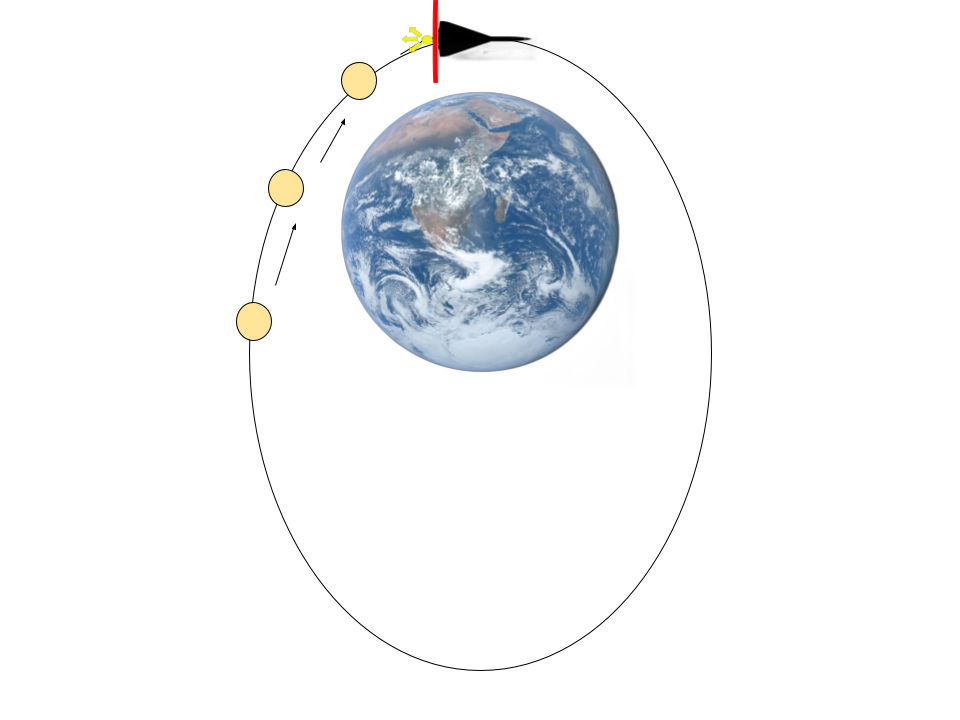
\includegraphics[width=0.5\linewidth]{images/Starship_Impact_ellipse.png}
    \caption{PuffSats from a first rocket (not shown) crash their gas puffs into a second target rocket, transferring momentum for propulsion. \cite{earth_image}}
    \label{fig:PuffSat_impact}
\end{figure}

Recent missions such as Proba-3 \cite{esa_proba_3} demonstrate that centimeter-scale formation flying works---at least in high-altitude orbits. Therefore, most PuffSat navigation and control tasks can be handled with robust model predictive control (MPC) \cite{veenmanrobust_proba3} and Kalman filtering (see \autoref{sec:neural_navigation}).  These classical techniques are data-efficient, easy to interpret, enable clear reasoning about system behavior, and offer formal performance and safety guarantees. For the more demanding conditions near low periapsis, classical control methods can be augmented with neural networks that warm-start control algorithms, learn from residual errors, and provide resiliency to lost PuffSats and other anomalies (see \autoref{sec:neural_navigation}).

This speculative white paper is a brainstorming exploration that could be followed by more rigorous analysis. If the ideas prove too advanced for near term implementation, they can instead serve as fodder for hard science fiction. The paper summarizes and updates some of the writings from my own blog, "Aim Is All You Need."\cite{aim2024}

\begin{table}[!htpb]
    \centering
    \caption{A checklist of grand challenges PuffSat pulsed propulsion can solve}
    \label{tab:applications}
    \begin{tabularx}{\textwidth}{|c|L|}\hline 
        \textbf{Safer Satellite Launch} & We'll launch expensive satellites and astronauts without strapping them to fragile extremely high propellant mass fraction rockets.   See \autoref{sec:starship_safelaunch}. \\\hline
        \textbf{Suborbital Transit} & We'll create a viable suborbital travel vehicle allowing passengers to take off from normal airport runways and reach anywhere in the world in less than 2 hours. Noise pollution near population centers will be no worse than it is with conventional aircraft.  See \autoref{sec:200_mile_high}.\\\hline
        \textbf{Rocket Revolution} & We'll end the tyranny of the rocket equation. We'll still use small rockets, but giant rockets with high propellant mass fraction will no longer be needed to reach orbit. See \autoref{sec:no_isru_rocket}\\\hline
        \textbf{Lunar Lift-off} & Launching from the moon may still require volatiles, but not the more difficult task of making and storing high performance rocket fuel.   See \autoref{sec:lunar_rockets_no_fuel}\\ \hline
        \textbf{Jurassic Dark} & As a side effect of our advances, we'll create the field of lunar cold trap paleontology and discover concrete evidence for how life originated on Earth. We'll build a genetic record of extinct species from ancient geological periods, like the dinosaurs. See \autoref{sec:jurassic_dark} \\\hline
        \textbf{Straw Ways To Heaven} & We can construct terrestrial megastructures, extending from the ground to the edge of space, without relying on advanced magnetic technologies such as Lofstrom Launch Loops \cite{lofstrom_loop}. A particularly ambitious yet beneficial example might be a vacuum tube connecting Earth and space, a "Straw Way To Heaven." See \autoref{sec:straw_way_to_heaven}.\\\hline
        \textbf{Carbon Cancelled} & We will solve our energy problems with carbon negative fuel that absorbs the carbon dioxide produced by industry, all while using minimal land and resources.  See \autoref{sec:death_star}.\\\hline
        \textbf{Moon Mining} & We'll develop in-situ resource utilization (ISRU) technology, first on our moon (See \autoref{sec:lunar_mining}),  and then on icy moons like Saturn's moon Phoebe (See \autoref{sec:greedy_phoebe}).  Ceres may also prove valuable for ISRU mining (See \autoref{sec:ceresly_good}).\\\hline
        \textbf{Cosmic Commutes} & We'll  build fusion powered spaceships with Earth-like artificial gravity that travel on brachistochrone trajectories with constant acceleration and deceleration between destinations.  \autoref{sec:epstein_drives}\\\hline
    \end{tabularx}
\end{table}
\end{abstract}.  

\section{Introduction}
Conceived in the 1950s and later popularized by \textit{The Three-Body Problem} \cite{liu2014three}, Project Orion remains one of the most compelling rockets ever proposed. It uniquely offers specific impulses surpassing those of electric propulsion while delivering thrust levels on par with chemical rockets \cite{projorion}.   Orion would propel a spacecraft by directing hypervelocity plasma from nuclear explosions onto a pusher plate. Despite its theoretical promise, Orion faced insurmountable challenges related to political feasibility, radioactive fallout, and the impractical mass requirements stemming from the high minimum yield of nuclear explosions. Nevertheless, Orion conceptually validated the physics of hypervelocity pulsed propulsion.   

Our approach replaces nuclear bombs with precisely aimed, hypervelocity gas puffs from specialized "PuffSat" microsatellites (see \autoref{sec:puffsat_design}) sequentially impacting a rocket's pusher plate.  These gas puffs can be scaled down to practical sizes.  Unlike nuclear explosions, small hypervelocity gas impacts could be efficiently contained within a pulsed propulsion chamber.

Leveraging gravity assists and the Oberth effect \cite{oberth_effect}, hypervelocity PuffSat impacts could achieve high energy densities and specific impulses.  Conventional control and estimation methods, which offer dependable results, can form the backbone of PuffSat guidance algorithms.  Neural networks optionally augment these systems by adjusting for unmodeled dynamics in complex orbital regimes and by reducing computational latency (see \autoref{sec:neural_navigation}).  

This speculative white paper presents a preliminary back of the envelope analysis of what are clearly very ambitious ideas. While rigorous, high fidelity modeling is left for future work, our aim is to stimulate fresh thinking and new research directions. Whether this concept remains a provocative thought experiment, inspires science fiction, or evolves into a transformative 21st-century technology, it underscores bold and novel applications of emerging formation flying capabilities. 

\section{Groundwork And Prior Work For PuffSat Pulsed Propulsion}
\subsection{PuffSat Formation Challenges Compared To Current Missions}\label{sec:formation_challenges_current_missions}
Centimeter-accuracy CubeSat formation flying is rapidly advancing. The European Space Agency's (ESA) Proba-3 mission recently demonstrated this capability by creating artificial solar eclipses with a precise two-satellite formation \cite{esa_proba_3}. The Stanford Space Rendezvous Laboratory's VISORS mission \cite{guffanti2023autonomous}, nearing flight readiness (as of September 2025), will showcase centimeter-precision formation flying with 6U CubeSats for \SI{10}{\second} durations at a \SI{600}{\kilo\meter} altitude \cite{visors_formation_flying}.

Our hypervelocity PuffSats employ formation-flying algorithms for precise positioning, but with a greater margin for error than VISORS or Proba-3. Those missions demanded sub-arcsecond pointing for imaging, whereas PuffSats can have wider rotational misalignments and still satisfy mission objectives. Likewise, the formation can probably accommodate pusher-plate impacts with a standard deviation of \SI{5}{\centi\meter} from the target center, easing lateral control constraints.

Operating at a lower interception altitude (\SI{200}{\kilo\meter}) introduces stronger and more variable drag perturbations than at VISORS' \SI{600}{\kilo\meter} orbit. VISORS maintains a near-circular sun-synchronous orbit and is therefore continuously exposed to peak drag, whereas PuffSats spend only minutes below VISORS' altitude. While PuffSats traverse low altitudes at higher speeds, their brief dwell time at these heights limits the accumulation of drag-induced drift.  Timing PuffSat interceptions at night, in colder regions, or during periods of low solar activity can reduce the atmospheric drag PuffSats experience during their descent.

GOCE, a substantially larger satellite, achieved full drag compensation at altitudes as low as  \SI{229}{\kilo\meter} using a streamlined aerodynamic profile coupled with \SI{20}{\milli\newton} ion thrusters \cite{goce_dragfree, goce_229km}. Though electric propulsion for CubeSats is actively being developed \cite{busek_iodine}, adapting GOCE's ion propulsion system for a PuffSat remains unrealistic due to mass and power constraints. However, PuffSats could be elongated like GOCE to reduce drag. Torque could be mitigated by modest spin stabilization or GOCE-like fins, combined with cold gas or small chemical thrusters for fine control.

GOCE demonstrated that small accelerometers can accurately measure atmospheric drag, enabling precise corrective maneuvers. Based on the crude GOCE-derived modeling discussed in \autoref{sec:estimate_cold_gas}, PuffSats using cold gas thrusters would expend at most \SI{400}{\gram} of propellant during descent through denser atmospheric layers below \SI{600}{\kilo\meter}, even with pessimistic assumptions. Estimated peak thrust requirements of approximately \SI{400}{\milli\newton} appear sufficient to counteract drag forces below VISORS' operational altitude. This conservative “back-of-the-napkin” estimate provides a very rough upper bound, with propellant for low-altitude drag cancellation comprising less than 2\% of a \SI{25}{\kilo\gram} PuffSat's total mass.

Cold gas thrusters, like all PuffSat components, must minimize dry mass to reduce impact risk with the pusher plate (see \autoref{sec:coordinator_node_dry_mass_disposal}). A conventional cold gas storage tank would likely need to be embedded within the PuffSat to protect it from micrometeoroid damage, which increases both volume and drag. These tanks are also typically expensive to manufacture and pose some risks of hitting the pusher plate as shrapnel.

An alternative approach is to replace the bulky tank with lightweight, thin bladders supplied by metered valves that release small amounts of gas-generating liquids.  Each bladder would transiently store gram-scale quantities of gas, providing propellant for fine-control thrusters. For example, a system might use a gram of water mixed with milligrams of green propellants like catalytically decomposed hydrogen peroxide to generate moderately heated, pressurized steam for gas thrusting. Small amounts of fuel may be added both to supply additional thermal energy and to react with harsh oxidizers in the exhaust stream.  Corrosion and residue are challenges in microfluidics. Fortunately, the very short, low-altitude peak operating times of the system partially mitigate these risks. We can also implement a hybrid architecture, where green propellants directly provide supplemental thrust bursts without intermediate bladders when thrust requirements approach the maximum of \SI{400}{\milli\newton}.

If the plumbing and support hardware for this microfluidic system weigh no more than \SI{50}{\gram}, the total dry mass would likely be lower than that of a standard \SI{400}{\gram} nitrogen tank. The compact geometry also reduces drag and makes ejection ahead of pusher contact more straightforward. As the thin polymer bladder skin fragments travel through the gas plume toward the pusher, they are decelerated and ablated, likely limiting impact damage to the pusher's ablative layers.  The increased complexity of microfluidics introduces the risk of catastrophic PuffSat failures. However, the system must already be resilient to PuffSat losses, given many are used on each launch.

Because PuffSats are single-use and operate for only half of a single orbit, we can budget more propellant for aggressive drag and torque correction. For PuffSats, overestimating propellant needs is wise. Unused gas hits the pusher plate, so it is not wasted—though variability in this leftover gas propulsion slightly complicates the intercepting rocket’s trajectory adjustments between impacts. The first few PuffSats to intercept the target rocket will experience the lowest altitudes (closest to \SI{200}{\kilo\meter}) before the rocket rises slightly as it accelerates towards orbit (see \autoref{sec:leo_orbit_details}). To optimize propellant usage, we can equip these initial units with slightly more propellant to compensate for their more challenging trajectory.

If control remains impractical, we can simplify by increasing the PuffSat interception altitude. If we raise interception to \SI{300}{\kilo\meter}, a reusable suborbital target rocket (see \autoref{sec:200_mile_high}) would require somewhat higher propellant mass fractions, suffer marginally greater re-entry heating, and benefit slightly less from PuffSat velocity. However, raising interception height may be an acceptable compromise if lower altitudes near \SI{200}{\kilo\meter} prove unmanageable.

\subsection{Coordinator Node Architecture And Dry Mass Disposal}\label{sec:coordinator_node_dry_mass_disposal}
To maximize gas mass while minimizing the non-volatile solid mass of the mini-thrusters and electronics, a small number of coordinator satellites with enhanced computing power will track the PuffSats' positions and relay adjustment commands.  The coordinator nodes will account for communications and PuffSat actuator latencies when determining PuffSat control trajectories.  As shown in \autoref{fig:coordinator-nodes}, these heavier coordinator nodes fly alongside the PuffSats but do not impact the target rocket. The PuffSats themselves carry only simple, low-mass electronics. Because hundreds of PuffSats are required per mission, mass production will help reduce overall costs.

Inspired by the smallest PocketQube pico-satellite designs \cite{pocketqube_mass_reference}, each PuffSat carries no more than \SI{250}{\gram} of dry mass.  This dry mass includes sensors, power systems, microthrusters, and low bandwidth communication links to the coordinator nodes.  If typical PuffSats carry more than \SI{25}{\kilo\gram} of fuel and propulsion mass, non-volatile solids constitute less than 1\% of their total mass. To prevent this dry mass from impacting the rocket, we propose several disposal strategies:

\begin{itemize}
    \item \textbf{Discard Before Impact:}  The dry mass components could launch slightly away from the rocket just before impact. If explosives are used to gasify the PuffSat (see \autoref{sec:explosive_puffsat}), shaped explosive sections can direct and accelerate the non-volatile solids radially outward at high speed.   The shaped explosives ensure the non-volatile solids  outrun the expanding gas envelope and clear the target radius prior to impact.  The shaped explosives also partially decelerate the solids, lowering their perigee to further reduce the risk of creating space debris (see \autoref{sec:handling_space_debris}). \label{item:discard_before_impact}
    \item \textbf{Active Elimination:} Equipment on the target rocket could obliterate the dry mass via electric discharges, directed energy beams, or sprays of material that hit the incoming PuffSat solids before pusher plate impact.
    \item \textbf{Passive Routing:} The dry mass components could pass harmlessly through a small aperture in the pusher plate.
\end{itemize} 

All of these impact mitigation techniques would occasionally fail.  In this case, the pusher plate itself serves as a last line of defense.   A strong, heat tolerant, Kevlar backed pusher plate (see \autoref{sec:lightweight_pusher_plates}) structurally resembles  Whipple shielding \cite{whipple_shield}.  The pusher plate would pulverize the non-volatile solids and prevent catastrophic damage to crewed compartments or high value satellites.  The target rocket would then ideally steer out of the PuffSat stream and abort.  If carrying people, the target rocket survives reentry with single-use but reliable ablative heat shields.  The target rocket might carry swappable, redundant pusher plates to allow for mission continuation following a single component failure.  Even with redundancy, we retain the capability for reentry in a  worst-case multiple-failure scenario.

\begin{figure}[htpb]
    \centering
    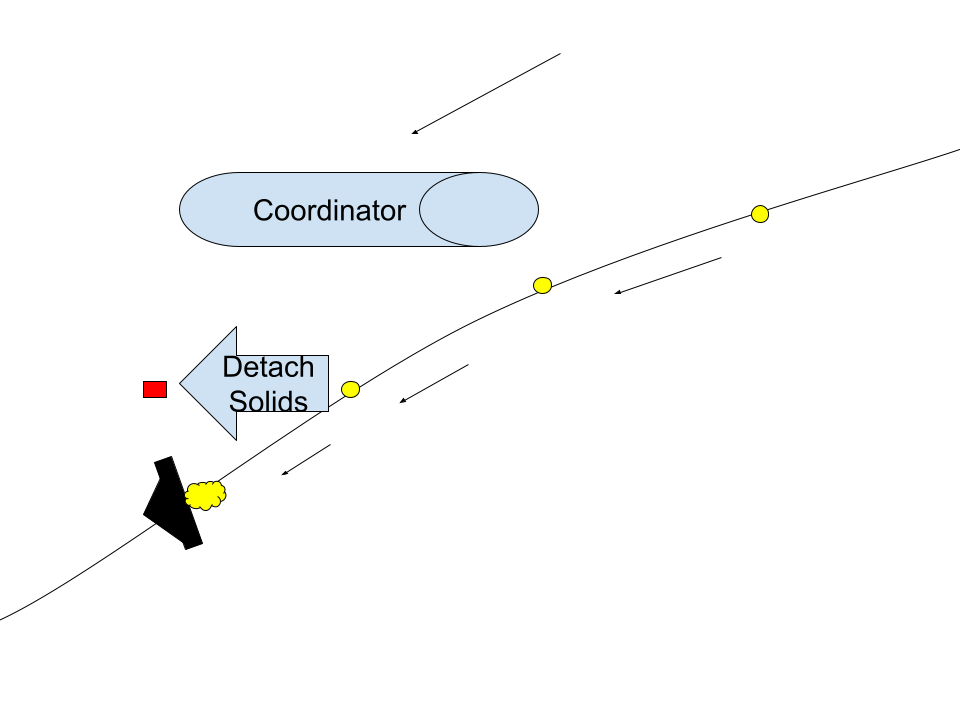
\includegraphics[width=0.5\linewidth]{images/Coordinator Nodes.png}
    \caption{Coordinator nodes (non-impacting) handle measurement and computation; PuffSat solids detach or pass through the pusher plate's aperture before impact.}
    \label{fig:coordinator-nodes}
\end{figure} 

\subsubsection{Steering PuffSats With High Powered Lasers}
Instead of relying on non-volatile solid components, radiation pressure could directly manipulate PuffSats. Coordinator nodes might employ kilowatt-class lasers to adjust PuffSat trajectories. The intense laser light could also induce temporary thermal or photochromic changes in the PuffSat's skin, altering its geometry or albedo. If these changes briefly persist, the altered solar radiation pressure would magnify PuffSat trajectory changes compared to the laser's radiation pressure alone. Eliminating non-volatile solid components on PuffSats  reduces the risk of pusher plate damage in an accident.  The PuffSats cost less without microthrusters and electronics. However, space lasers present several drawbacks compared to microthrusters. They exert weak forces on the PuffSats, demand substantial power sources for coordinator nodes, and are not yet a fully mature technology. 

\subsection{A Rough Sketch Of The Software Guidance For PuffSat Interception}\label{sec:neural_navigation}
To ensure a precise interception of the next PuffSat, the target spacecraft's rocket-based reaction control system must rapidly adjust its trajectory. It must do this within fractions of a second after each impact, correcting for the difference between the expected and actual momentum transfer from the previous PuffSat.  A prerequisite for these hypervelocity PuffSat rendezvous is accurately capturing the position and velocity of the PuffSats.  For this, a standard Unscented Kalman Filter (UKF) \cite{wan2000unscented} offers robust state estimation when dynamics are well-modeled and noise is Gaussian.  The large formation of PuffSats provides a dense measurement stream, further improving filter performance.  

PuffSat interceptions, however, may occur near low periapsis in denser atmospheric layers where drag, gravitational anomalies, sensor dropouts, and outliers challenge UKF's assumptions and accuracy.  When such effects become significant, state estimation could be improved with hybrid approaches that augment the UKF with neural networks that learn residuals on real and simulated orbital data \cite{takigawa2023comparison}.  For example, methods like KalmanNet \cite{revach_2022_kalmannet} \cite{revach2022unsupervised} have shown robustness to unmodeled disturbances in simulations.  Neural inference scales favorably compared to Kalman filtering, especially as the number of states estimated grows.  As a result, neural estimators may support more frequent updates in a large PuffSat formation.  

Verifiable, data-efficient, interpretable techniques like model predictive control (MPC) can replan trajectories to correct for momentum prediction errors after PuffSat impacts.  Neural networks can  warm-start conventional tools with good initial guesses to reduce solve times, \cite{guffanti2024transformerstrajectoryoptimizationapplication} especially when there are many real-time constraints  \cite{briden_constraint}.  However, the control law itself could remain grounded in well-understood optimization and stability guarantees.     

Since conservative approaches appear feasible, we've prioritized them over faster, more opaque methods, such as parallel deep learning ensembles optimized for inference speed. That said, these black-box strategies merit consideration, as the risk of hardware failures in our PuffSat system may be no less significant than the risk of persistent control hallucinations in sufficiently large, diverse model ensembles.  In fact, reinforcement learning shows promise for developing fast space trajectory recovery algorithms for anomalies like lost PuffSats \cite{zavoli2021reinforcement} --- an area where standard control techniques struggle.  

While PuffSat navigation enables centimeter-scale centering in front of the pusher plate prior to detonation, gas generation unfolds over a finite duration and lacks comparable precision along the thrust axis. Nevertheless, centimeter-level lateral positioning ensures that the plume impinges symmetrically---preserving the target vehicle’s inertial stability.  The target rocket's reaction control system would still need high performance to cancel undesirable torques from the occasional PuffSat that hits the pusher plate significantly off-center.

\subsection{PuffSat Design And Gas Generation Details}\label{sec:puffsat_design}
The optimal PuffSat design depends on the launch scenario and mission requirements.  
\subsubsection{Explosive PuffSats} \label{sec:explosive_puffsat}
Explosive PuffSats are engineered to detonate at a precisely calibrated standoff distance from the pusher plate. This timing ensures rapid conversion of their mass into a high-velocity gas plume, shaped to distribute momentum evenly across the plate surface.  To minimize aerodynamic drag during flight, each PuffSat adopts an elongated cylindrical geometry aligned with the direction of travel (see \autoref{sec:formation_challenges_current_missions}). This shape also extends the duration of gas-plume interaction, slightly reducing peak stress on the pusher plate without significantly compromising momentum transfer efficiency. A small shaped section of the PuffSat's explosive charge can also eject non-volatile solid components away from the rocket before impact, as described in \autoref{item:discard_before_impact}.  A failure to detonate at the intended moment could damage the pusher plate or the rocket, so redundant initiation systems are essential.

As shown in \autoref{fig:explosive_puffsat}, each PuffSat carries its own detonation system. As a backup to ensure reliable triggering, the rocket emits a sparse layer of volatile material (e.g., water ice) a few meters ahead of the pusher plate just before each PuffSat arrives. Passing through this ice layer produces a shock that guarantees detonation. The geometry precludes a  PuffSat from reaching the rocket without first crashing through its ice layer. To minimize mass, the layers can be prefabricated as a sparse lattice or parallel wires. For instance, parallel ice wires with square \SI{500}{\micro\meter} cross sections  spaced \SI{5}{\centi\meter} apart have an areal density of only $\SI{20}{wires\per\meter} \times (\SI{500}{\micro\meter})^2 \times \SI{917}{\kilo\gram\per\cubic\meter} \approx \SI{5}{\gram\per\square\meter}$.  To improve handling and tensile strength during deployment, the ice wires can be coated with a micron-thin layer of metal or plastic. The coating needs to be light enough for orbital drag to deorbit it quickly, and thin enough that it doesn't pose a major collision hazard to other satellites. Additionally, the coatings must avoid toxic elements like fluorine, because they'll be vaporized upon impact.  

If frozen materials prove impractical, the wires could instead be constructed from low-mass plastic explosives, designed to detonate on PuffSat impact.  If the rocket misses a PuffSat interception after reaching  minimum orbital speed, the explosive wires would unfortunately become space debris. This debris could  persist for hours or days until eroded by atomic oxygen or slowed enough by atmospheric drag to re-enter. Another alternative is to replace ice wires with liquid sprays that induce a shock detonation of the PuffSat’s explosives upon impact.

\begin{figure}
    \centering
    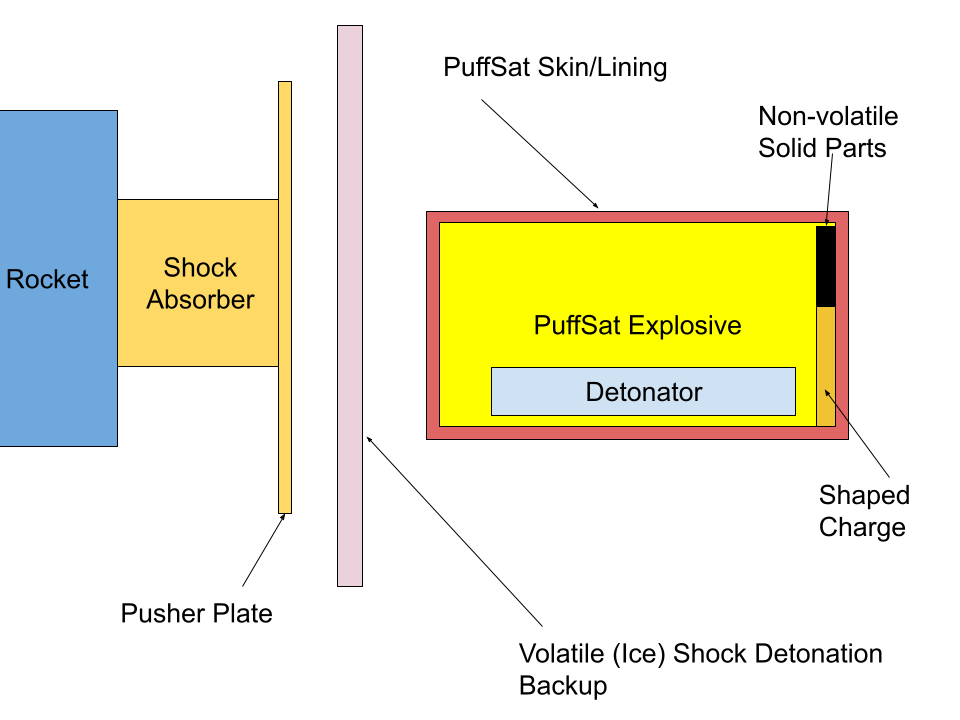
\includegraphics[width=0.5\linewidth]{images/Explosive PuffSat.png}
    \caption{Cross sectional diagram of the key parts of an explosive PuffSat}
    \label{fig:explosive_puffsat}
\end{figure}

This paper does not attempt to identify optimal explosive chemistries. That selection entails complex trade-offs in sensitivity, handling safety, cost, and environmental impact—issues more appropriately addressed in applied engineering contexts than in conceptual mission design. For modeling purposes in \autoref{sec:estimate_cold_gas}, we adopt ANFO \cite{wikipediaANFO} as a shock-insensitive, deliberately unsuitable proxy. Its low density increases drag for a given PuffSat mass, helping ensure our performance estimates remain conservative while avoiding dual-use implications.

To prevent outgassing, the PuffSat's explosives are encased in very thin layers of high performance polymers or metals. These liners can also reflect sunlight, further reducing temperatures to minimize the escape of volatile materials. The skin could contain a thin foam that prevents shock detonation from micrometeorites smaller than \SI{5}{\micro\meter}.  However, the skin should not be thick enough to protect against shock detonation from the ice wires we use as a detonator backup.  Significant micrometeorite impacts simply result in PuffSat losses.   Explosive PuffSats are ideal for terrestrial launches, where the necessary chemicals are relatively easy to manufacture.

\subsubsection{Solid Ice Based PuffSats} \label{sec:icy_puffsat}
PuffSats filled with lunar ice (see \autoref{sec:lunar_rockets_no_fuel}) do not primarily rely on chemical reactions to produce gas. Their high tensile skins absorb sunlight, melting the ice to water under mild pressure. Small explosives or an ice wire impactor (see \autoref{sec:explosive_puffsat}) rupture the skin to release the water. However, this release is too slow for complete vaporization before impact, and full vaporization would cool the steam so rapidly that ice crystals would form.

Instead, the water is atomized into fine droplets, a process requiring much less energy than vaporization. To drive atomization, microscopic explosive particles are suspended in the water, either as a colloidal slurry or encapsulated in microbubbles.  The resulting mixture resembles a low-density explosive emulsion—not unlike the water-based emulsions used in terrestrial mining and construction \cite{emulsion_tutorial}, but significantly diluted and tuned for spaceflight safety.

Unlike industrial emulsions designed for high-yield detonation, our explosive concentration is just sufficient to atomize the water. This approach maximizes ISRU-derived water mass while minimizing risk. Sensitizing agents from a separate bladder inside the PuffSat can be mixed  with the main explosive liquid mass late in the PuffSat’s flight to prevent premature activation, allowing the system to remain stable during launch and transit.  

In microgravity, thermal agitation induces Brownian motion, naturally yielding a stochastically mixed, quasi-uniform explosive particle distribution. These micro-explosives are chosen for precise shock sensitivity, ensuring they detonate upon high velocity impact with the incoming ice layer or in response to the main rupture charges. While likely imported from Earth due to manufacturing complexity, the micro-explosives' total mass is small compared to the bulk water payload.

Additional ice particles injected by the rocket ahead of the plume induce energetic turbulent mixing. The resulting aerodynamic shear, combined with micro-explosive detonations, fully atomizes the water into fine droplets before it reaches the rocket’s pusher plate.

\subsubsection{Liquid Oxygen PuffSats}\label{sec:lox_puffsat}
PuffSats filled with lunar oxygen (see \autoref{sec:lunar_mining}) must also atomize before reaching the pusher plate. To retain liquid oxygen during orbital transit, these PuffSats require thicker skins engineered for elevated internal pressures, cryotolerance, and thermal insulation. To minimize boiling of the highly pressurized LOX (liquid oxygen), PuffSats use high-reflectivity coatings such as emerging "solar white" yttrium oxide composites (see \autoref{sec:epstein_drives}).  These coatings are backed by emissive layers that radiate residual heat into space, maintaining cryogenic temperatures without active cooling.

Upon rupture, the thicker skin risks becoming hazardous shrapnel. While PuffSat skins are engineered to retain cryogenic LOX under elevated internal pressure, they need not be shock-resistant (though an outer protection against micron-scale micrometeorites is still required). In fact, selecting materials prone to brittle fracture at low temperatures may enhance debris mitigation by ensuring the skin fragments on impact. The rocket releases a denser intercepting ice layer that shatters the brittle skin in a process analogous to how Whipple shielding breaks up space debris into less threatening dust \cite{whipple_shield}.

As with the icy PuffSats discussed in \autoref{sec:icy_puffsat}, the liquid oxygen is atomized through a combination of micro-explosive detonation, aerodynamic shear, and shock interaction with the ice layer.  Note that the pusher plate for liquid oxygen PuffSats must be lined with a non-combustible material.

\subsubsection{Balloon PuffSats}
Inflated balloon PuffSats avoid the catastrophic risk of failed detonations.  When filled with gaseous water vapor or oxygen, balloon PuffSats can operate without advanced reflective cooling. Project Echo \cite{JPL_EchoQL2010} demonstrated that large orbital balloons can be built from low-cost materials such as metalized mylar.

At low periapsis, maintaining balloon navigation control and structural integrity is difficult because of  atmospheric drag, debris impacts, and radiation pressure. Large balloon surface area also demands more polymer, increasing costs significantly. If high performance polymer costs drop substantially, balloon PuffSats could become a favorable option.

\subsection{Comparison To Pellet Beam Propulsion Prior Art}
In 2001, Gerald Nordley proposed an externally pulsed propulsion system in which hypervelocity pellets, capable of self-steering, transfer momentum to a spacecraft via impact with a pusher plate \cite{nordley2001interstellar}. This concept built upon earlier work by Clifford Singer \cite{singer1979interstellar}, who envisioned unguided macroscopic projectiles launched at extreme velocities. 

Both Singer’s and Nordley’s designs relied on mass drivers.  These devices would need to accelerate sizable objects to very high speeds, posing formidable engineering challenges. To address this, Jordan Kare introduced the SailBeam concept \cite{kare2001sailbeam}, which replaced the mass driver with solar or laser driven miniature sails. Kare further proposed vaporizing the sails upon impact and using a magnetic pusher plate to convert the resulting plasma into thrust.   Artur Davoyan received NASA funding to improve the efficiency of Kare's ideas by accelerating pellets using laser ablation rather than radiation pressure alone \cite{davoyan2023pelletbeam}.

These pellet stream propulsion ideas often prioritized interstellar speeds over economic feasibility.  Instead of using expensive mass drivers or light sails, our PuffSat pulse propulsion system focuses on achieving high speeds primarily through low cost orbital maneuvers.  Unlike pellet beam proposals, PuffSat pulsed propulsion aims to  provide very heavy lift to propel large craft into orbit.  These pellet beam proposals also generally don't seriously examine near-term power sources capable of lifting multi-ton objects into orbit. Our PuffSats can weigh kilograms, and are composed mostly of materials that gasify to biocompatible chemicals like water vapor, nitrogen, oxygen, and carbon dioxide.   This means they generate substantially less pollution for a given $\Delta V$ (delta-v), which makes them practical for very large-scale near-Earth applications.  

Although our PuffSats contain electronics, the majority of their mass consists of inexpensive explosives or ices. This composition enables comparable propulsion at significantly lower cost than systems dominated by electronics or solar sail material. Water ice, in particular, is abundant and mineable throughout the solar system.  Larger PuffSats can afford heavier electronics than Nordley's snowflake sized guided pellets.  While PuffSats could, in principle, interact with magnetic pusher plates, their largely gaseous composition (after gas generation) may make direct kinetic collision a simpler and more robust mechanism for momentum transfer.  However, magnetic technologies would still be useful in the shock-absorber behind the pusher plate (see \autoref{sec:lightweight_pusher_plates}).  If a dense flow of small pellets hits a rocket, the resulting plumes may interfere with each other.   PuffSats have larger pulses spaced far enough apart that plume interference is neglibible.

\subsection{Mass Fraction Of Rocket To PuffSat Mass}
For PuffSat pulsed propulsion to be a viable option, the ratio of PuffSat gas mass to target rocket mass must be low for relevant rocket velocity changes. We develop a closed-form approximation for this ratio ( \autoref{eq:PuffSat_ratio} in {\autoref{sec:PuffSat_ratio_approximation}). Since real collisions are not perfectly elastic, our approximation includes an energy loss "fudge factor," $f$.  Justification for a high $f$ value comes from findings of Project Orion. The Orion team determined that collisions involving the pusher plate could be opaque  \cite{orion_reflections}. This opacity is a consequence of Kramers' opacity law \cite{kramers1928diffusion}, which states that opacity increases sharply with density. The plasma in the pusher plate is orders of magnitude denser than the low-density, inelastic plasma collisions studied in fields like fusion research.  Opacity implies minimal kinetic energy loss to pusher-plate heating, resulting in a more elastic impact. Pusher plate durability and opacity could be further enhanced by spraying a thin layer of dark ablative material  on the plate between impacts (see \autoref{sec:lightweight_pusher_plates}).   Additionally, a curved, roughly parabolic pusher plate would produce a  highly collimated gas reflection. A fudge factor of $f=0.5$ is perfectly inelastic, but with all gas hitting the pusher plate. Perfectly elastic collisions correspond to $f=1$.  We select a high $f=0.8$, though the mission scenarios this paper discusses are still viable with more conservative fudge factor values.   

Relevant mass ratios and mission scenarios are summarized in \autoref{tab:mass_scenarios}. This table clearly shows that PuffSat pulsed propulsion can lift significant mass into orbit. For instance, if a reusable rocket like SpaceX Starship \cite{starship} lifts \SI{25}{\tonne} of PuffSats into a trans-lunar orbit, they can propel a  \SI{32}{\tonne} target craft into low Earth orbit. This exceeds the Space Shuttle's maximum capacity \cite{space_shuttle_program} or the zero fuel mass of smaller regional jets like the Embraer E170 \cite{embraer_e170}.

\begin{table}[!htpb] % tabularx should be inside a table environment
    \centering
    \caption{Mass ratio of rocket to PuffSat with fudge factor \(f=0.8\) \cite{Katz_aim_is_all_you_need_2025}}
    \label{tab:mass_scenarios}
    \begin{tabularx}{\textwidth}{|p{4em}|p{4em}|p{4em}|p{6em}|L|}\hline
        \textbf{Rocket
        Final
        Velocity
        (\SI{}{\km\per\second})} & \textbf{PuffSat
        Velocity (\SI{}{\km\per\second})} & \textbf{Rocket
        Initial
        Velocity (\SI{}{\km\per\second})} & \textbf{Rocket/PuffSat
        Mass
        Ratio} & \textbf{Scenario} \\\hline
        7.784 & 10.916 & 0 & 1.28 & Eccentric PuffSats with apogee at lunar distance pushes rocket to minimal low Earth orbit. See \autoref{sec:starship_safelaunch}\\\hline
        0 & -7.784 & 7.784 & 2.308 & Decelerate intercity rocket for powered reentry with retrograde PuffSats in low orbit.  See \autoref{sec:200_mile_high}\\\hline
        0 & -10.916 & 7.784 & 2.97 & Decelerate intercity rocket for powered reentry with retrograde PuffSats from lunar orbit. See \autoref{sec:200_mile_high} \\\hline
        23.66 & 69.272 & 0 & 3.83 & PuffSats approach Earth from Jupiter retrograde Hohmann trajectory and push the object to escape velocity and then to a periapsis near Parker Space probe.  See \autoref{sec:jupiter_gravity_initial} \\\hline
        40.17 & 69.272 & 0 & 1.85 & PuffSats approach Earth from Jupiter retrograde Hohmann trajectory and push the object to escape velocity and then to a periapsis near Parker Space probe but in a retrograde orbit around the Sun. See \autoref{sec:jupiter_gravity_initial} \\\hline
        10.916 & 69.272 & 0 & 9.331 & PuffSats approach Earth from Jupiter and push a rocket into an elliptical orbit.  See \autoref{sec:jupiter_only_growth} \\\hline
        3 and 3.7 & 7.20 & 0 & 1.455 & Launch PuffSats from the moon to trans-lunar injection orbit with low periapsis on Earth.  See \autoref{sec:lunar_rockets_no_fuel} \\\hline
        0 & -2.38 & 2.38 & 2.30 & Decelerate trans-lunar payloads to land on the moon, ignoring the moon's speed around Earth.  See \autoref{sec:no_isru_rocket} \\\hline
        24.98 & 35.25 & 0 & 1.29 & PuffSats approach Saturn from Phoebe and push a helium-3 payload into a temporary very low orbit around Saturn.  See \autoref{sec:mining_helium_3} \\\hline
    \end{tabularx}
\end{table}

\subsection{Handling Space Debris} \label{sec:handling_space_debris}
The dry mass components of each PuffSat risk becoming space debris. To avoid this, we can intercept the PuffSats prior to their orbital periapsis.   For example, a PuffSat interception at a \SI{200}{\kilo\meter} altitude likely follows a predictable trajectory with negligible atmospheric drag.   If the PuffSat periapsis is near \SI{50}{\kilo\meter}, this likely deorbits any dry mass components.   They ideally then burn up or fall over remote oceans.  PuffSats that miss their target rockets either boil or explode from reentry heating, eliminating the risk of heavy debris reaching the ground. Two other techniques prevent long-lasting space debris:

\begin{itemize}
\item The J2 perturbation induces a changing argument of periapsis. Any PuffSat orbit designed to avoid specific critical angles will eventually have a periapsis over the equator.  Since the Earth is wider at the equator, periapsis will be at a lower atmospheric altitude with much more drag.
\item If our PuffSat interceptions occur at night, subsequent daytime periapsis will be over a warmer atmosphere with higher drag at the same altitude.
\end{itemize}

Since PuffSats form large formations, care must also be taken to avoid existing satellites.  Short, seconds-long gaps in the formation could be intentionally introduced to avoid collisions.

\subsection{PuffSat Deployment Details For Low Earth Orbit Scenario}\label{sec:leo_orbit_details}
Let's consider the complexities of launching target rockets into Low Earth Orbit (LEO) with propulsion from PuffSats deployed in highly eccentric Earth orbits.

It's crucial to acknowledge that these PuffSats will not follow strictly identical Keplerian orbits. As the target rocket accelerates, the optimal PuffSat interception point moves along with it, so that successive PuffSats have slightly different orbital elements.
For low-mass PuffSats, solar radiation pressure will significantly distort their orbits. To simplify orbit planning and maintain consistent  effects across the fleet, it's ideal for each PuffSat to remain outside the shadow of the others. This may necessitate slight variations in orbital parameters, such as inclination, for nearby PuffSats. The micro thrusters on each PuffSat  make corrections for unmodeled perturbations.  We still ensure each PuffSat achieves the correct interception position with the target rocket.   

Fortunately, deploying PuffSats near apoapsis strategically minimizes the $\Delta V$ required for both inclination changes and optimal satellite spacing. This reduction in required thrust suggests that mechanical launchers with moderate size, power and peak acceleration could deploy PuffSats very precisely with sufficient velocity changes.  The launch mechanism could use rotating wheels or computer-controlled rail catapults, with recoil forces countered by the rocket's reaction control systems. PuffSats can be launched in series, further reducing launch mechanism operational demands.

\subsection{Lightweight Pusher Plate Design: Materials and Damping Innovations Beyond Orion}\label{sec:lightweight_pusher_plates}
Modern material science enables pusher plate architectures far lighter than those contemplated by Project Orion. Although individual PuffSat pulses may reach peak shock pressures comparable to Orion’s nuclear impacts, their total impulse is orders of magnitude lower. This reduced force permits thinner structural elements—analogous to how rifle barrels withstand high pressures with far less mass than \SI{155}{\milli\meter} artillery barrels. Unlike Orion, PuffSat plates don't need to shield crew from nuclear radiation.  The absence of bomb radiation also extends longevity for pusher plate materials like complex aramid polymers.

Kevlar liners, unavailable during Orion’s development, offer lightweight spall protection against impact fragmentation \cite{spall_liners}. Titanium alloys, such as those used in the M777 Howitzer, demonstrate resilience under repeated pressure shocks and are viable candidates for structural plate substrates \cite{titanium_m777}. Fracture and corrosion resistant silicon nitride liners, currently studied for gun barrel applications \cite{silicon_nitride_gun}, could serve as a protective interface in PuffSat pushers.  Silicon nitride liners mitigate chemical corrosion across different PuffSat gas chemistries, including pure, superheated oxygen (see \autoref{sec:lox_puffsat}).  Temperature-resistant superalloys like Inconel 718 \cite{inconel_718_strong} can supplement or replace titanium where heat or cost justify the additional weight penalty.

An alternative architecture draws inspiration from Project Medusa \cite{solem_medusa}, a conceptual successor to Orion. Medusa replaced Orion’s rigid plates with flexible, parachute-like tensile sails. Scaled-down, high-tensile fabric sheets could absorb PuffSat impulses with reduced mass and simplified deployment above the atmosphere. Since PuffSats approach from the rear, these flexible pushers would be mounted behind the rocket on shock-absorbing struts. One candidate for the struts might be thermally-coated, reinforced carbon fiber with titanium or superalloy joints.  Carbon fiber offers high strength-to-weight and thermal stability, while advanced metal alloys prevent fracture at peak shock points.  In contrast to Medusa’s massive nuclear parachutes, PuffSat-compatible sheets can be thicker yet remain flexible, tailored to smaller impulse magnitudes. These fabrics may be shielded from corrosion and thermal loads by applying flexible coatings, such as those made from ceramic matrix composite yarns \cite{flexible_ceramic_composites} or high-temperature silicone \cite{silicon_coatings}.

Project Orion proposed that sacrificial ablative oils pre-applied to the pusher's skin would fully protect it from plasma vaporization \cite{orion_reflections}.   However, PuffSat gases like pure oxygen, carbon dioxide and water contain oxygen and will decompose at impact temperatures.  This oxygen would aggressively attack flammable ablators like PICA-X \cite{picax_ablator}.   Adding flame retardants and materials like boron carbide and hafnium carbide significantly increases the oxygen resistance of phenolic resins like PICA-X \cite{picax_flame_resistance}. Even so, the extreme conditions may make the non-flammable "solar salts" used for solar storage superior  \cite{hitec_solar_salt} ablators. Solar salts can absorb large amounts of thermal energy and decompose at temperatures far below the thermal failure point for advanced metal alloys or ceramic composites.  Solar salts become oxidizers when they decompose, but the resistant ceramic yarn or silicon nitride liners we discussed should withstand corrosion. Whether we choose brittle solar salts or PICA-X based ablators, they can both be embedded as micro particles in single-use flexible ceramic yarn felts so they stick to deformable Medusa-style pushers. 

Additionally, since there are no nuclear bombs subjecting semiconductors to extreme radiation, Puffsats can use large parallel arrays of space-qualified inkjet-style MEMS to evenly deposit micron-thick layers of ablative liquids across the pusher plate. The ablative materials could be silicone-based, organic oils, or ionic liquids.  In a vacuum, each droplet follows a predictable ballistic path, eliminating the need for bulky robotic sprayers. This path must account for transient accelerations imparted by the shock absorber system, as well as any impulse vectors from reaction control system firings, but remains precisely calculable in vacuum.  If the sprayed ablative is only 1 or 2 microns thick, the total mass is likely \SI{100}{\gram} or less for a \SI{25}{\square\meter} plate. These coatings can be formulated to vaporize under peak impulse heating, sacrificing themselves to protect the permanent pusher plate structure.

As opposed to Orion, our propulsion system includes reaction control thrusters (see \autoref{sec:neural_navigation}). These can be positioned forward on the target vehicle, increasing standoff distance and minimizing thermal or directional interference with the pusher plate. 

Shock absorber technology has advanced dramatically since Orion. Smart magnetorheological (MR) fluids offer dynamic vibration damping, reducing the risk of carbon fiber strut fracture under repeated loading \cite{mr_fluids}. To further reduce mass and thermal buildup, magnetic braking systems can complement mechanical springs and hydraulics. Rare-earth magnets \cite{rare_earth_braking} or high-field REBCO superconducting tapes \cite{rebco_tapes} enable compact, high-performance magnetic dampers previously infeasible. REBCO tapes are, however, still an emerging technology and require cryogenic refrigeration and superconductor quench management.  Because PuffSat impulses are scalable, we can deliberately reduce acceleration per pulse, further relaxing shock absorber requirements.

In sum, the absence of nuclear radiation, reduced impulse magnitudes, and modern advances in materials and damping systems enable lightweight, modular pusher plate designs tailored for PuffSat pulsed propulsion.

\section{To The Moon by Smart Gas Balloon:  The Business Case For PuffSat Pulsed Propulsion}   

\subsection{Making Starship's Excess Capacity Useful To Satellite Customers} \label{sec:starship_safelaunch}

SpaceX's Starship may be the first fully reusable rocket. At scale, this could dramatically reduce space flight costs.   However, the rocket's large payload size is probably too big for today's space industry needs. For example, in \textit{The New York Times}

\begin{quote}
Carissa Christensen, the chief executive of Bryce Tech, an analytics firm that tracks the launch market, says launching Starship frequently will be key to closing SpaceX’s business case, but finding customers to fill the rocket’s giant payload capacity will be challenging. 
"Starship's payload capacity is huge; it's very, very big, and there aren't that many commercial uses today for a rocket that big," she said.  "Maybe it'll be so cheap that it makes sense to launch satellites on it if it's not full or near full."  \cite{nyt_starship_size}
\end{quote}

Although many satellites might be too small to fill up Starship, they can still be very expensive to build and test. For an extreme example, the James Webb Telescope \cite{james_webb_space_telescope} cost \$9.7 billion dollars \cite{jwst_cost} to build. \textit{McKinsey Consulting} argues 

\begin{quote}
Safety and reliability will continue to be overarching concerns, suggesting excellent execution will be table stakes for a competitive launch company. \cite{mckinsey_reliability}
\end{quote}

Once rockets start ferrying astronauts, reliability becomes even more emphatically non-negotiable. Fully stacked, Starship weighs \SI{5}{\kilo\tonne} at launch \cite{starship}, yet its empty mass is only \SI{300}{\tonne}. That’s an awfully thin soda can strapped to a \SI{5}{\kilo\tonne} bomb that we're entrusting with billion dollar satellites or human passengers.

By contrast, a suborbital rocket that merely reaches \SI{200}{\kilo\meter} in altitude might have a propellant mass fraction under 60 percent. This greater structural margin allows for more robust, reliable engines and extensive payload protection systems. Of course, such a suborbital rocket cannot reach orbit on its own.  It needs Starship to "push" it with PuffSat pulsed propulsion.

\begin{figure}[htpb]
    \centering
    
\includegraphics[width=0.5\linewidth]{images/new_push_picture.png}
    \caption{A fun and of course very technically accurate cartoon about a suborbital rocket's $\Delta V$ limitations}
    \label{fig:suborbital-cartoon}
\end{figure}

Starship launches PuffSats for pulsed propulsion into a highly eccentric orbit around Earth, with a low \SI{50}{\kilo\meter} perigee and a high apogee (See \autoref{sec:handling_space_debris}). These PuffSats move near Earth’s escape velocity at their roughly \SI{200}{\kilo\meter} interception altitude. The suborbital rocket rides the PuffSats'  momentum pulses to low Earth orbit. While this approach reduces payload capacity compared to a single rocket system, most satellites are unable to take advantage of Starship’s enormous payload volume anyway.

\subsection{The 200 Mile High Club} \label{sec:200_mile_high}
SpaceX proposes direct Earth-to-Earth travel \cite{earth_to_earth}, ballistically launching passengers directly between cities with Starship from offshore platforms. This idea faces significant challenges:
\begin{itemize}
\item \textbf{Marine Environmental Impact:} Noise pollution from sea launches could severely harm marine ecosystems, including dolphins and whales.
\item \textbf{Noise Over Populated Areas:} Starship's descent would generate loud sonic booms over cities.
\item \textbf{Logistical Inefficiency:} Offshore launch platforms, by necessity located far from land, would add hours to the journey for boarding and departure, undermining the benefit of rapid travel.
\end{itemize}
A suborbital rocket plane offers a more practical alternative. To reach orbit, the suborbital rocket requires propulsion PuffSats launched by the Starship.   Starship can be launched from remote locations where noise pollution is acceptable.  Our suborbital rocket plane could take off from conventional urban airports using standard aircraft engines, then switch to rocket propulsion at high altitudes over remote areas to "skip" above the atmosphere and intercept Starship's propulsion PuffSats.   While normal airports can handle kerosene or methane fuel, most lack the infrastructure for cryogenic liquid oxygen.

However, two solutions address the liquid oxygen challenge:
\begin{itemize}
\item \textbf{Air-breathing Scramjets (Optimistic Scenario):} If economical passenger scramjets become feasible, rockets could accelerate to around Mach 7 before a steep climb, eliminating the need for liquid oxygen. This would also reduce propellant mass. Unfortunately, the extreme stress on the airframe makes suborbital rockets more economically viable for the foreseeable future.
\item \textbf{Mid-air Oxygen Refueling:} Suborbital rocket planes could receive liquid oxygen from specialized aircraft launched from airports equipped with liquid oxygen storage. This avoids retrofitting every urban airport, requiring only a single, strategically located airport near major destinations.   Mid-air refueling also reduces our rocket plane's takeoff weight.  Oxygen refueling would require research and development to create rigid cryotolerant pumps and docking mechanisms, distinct from the flexible hoses used in military operations today.
\end{itemize}

A formation of propulsion PuffSats launched in an eccentric Keplerian orbit could only propel the  rocket plane on trajectories that bisect the Earth. Since most urban destinations would not align with such trajectories, the rocket plane needs to fire an adjustment burn at least once to reach the destination. Alternatively, a second set of propulsion PuffSats could intercept the rocket plane mid-flight and adjust its trajectory. Furthermore, to avoid a sonic boom upon descent, the plane must decelerate before atmospheric reentry. This deceleration could be provided by yet another set of propulsion PuffSats that were traveling in a retrograde orbit relative to the plane. These reentry PuffSats could be in a circular low Earth orbit rather than a high eccentricity orbit, significantly reducing the mass required.

\subsection{What to Expect When You're Expecting Bodily G-Force}\label{sec:pregnant_women}\cite{expecting_pregnancy_book}
Pregnant women are prohibited from piloting fighter jets due to both safety and ethical concerns. Elevated G-forces and the extreme physical stress from using an ejection seat pose serious risks to the pilot and the developing fetus \cite{pregnancy_gforce_risk}. Suborbital transit, like military aviation, involves high, sustained accelerations.  Finding safe means to accommodate these vulnerable populations would help suborbital transit become mainstream.  The most straightforward mitigation is to reduce peak acceleration, but there are limits to this strategy.  Because of gravity losses, lower accelerations increase the $\Delta V$ required for a given trip.  

One promising technique is to seat passengers so that forces act chest to back along the body’s $Gx$ axis.   FAA guidance and pilot experience suggest this  force is generally well tolerated in healthy non-pregnant pilots \cite{lateral_acceleration}.  The FAA advisory also mentions that forces directed from the feet towards the head ($Gz-$) are the most dangerous for adults.   Babies frequently are oriented head down in the womb, although fluid buoyancy ameliorates the effects.    If the fetus tolerates the worst possible g-force direction, the tentative hypothesis is they can tolerate 2 g forces in the direction adults find most benign.  Neck pillows and back supports can comfort infants and adult passenger.  While the rocket's pusher plate reduces vibrations, infants may also need seats designed to provide additional protection against shaking.

Unfortunately, I found no studies directly evaluating the safety of even moderate (2 g) $Gx$ acceleration for pregnant women or infants. It's imperative we test safety protocols with  multi-stage trials.   These trials can initially test on mice and then progress to non-human primates.  Since human babies have larger brains, only tests on human subjects can truly confirm they are not harmed when following acceleration mitigation procedures.  If we can't confidently establish that suborbital flight is completely benign, these groups must be excluded from suborbital flights.  

\section{I Love ISRU.  Cheaper PuffSat Pulsed Propulsion \textit{Without} Giant Reusable Rockets}
For PuffSat pulsed propulsion of intercity passengers to achieve genuine economic competitiveness, the cost of launching  propulsion PuffSats must be exceptionally low.  The rocket plane must be robust enough to guarantee on-time takeoffs and avoid missing its initial PuffSat rendezvous.  Rocket acceleration and passenger cabin vibrations must be limited for infants and other susceptible passengers (see \autoref{sec:pregnant_women}), further increasing costs and $\Delta V$.  Even highly reusable rockets may prove too expensive, limiting this technology primarily to the very high-end private luxury aviation market. While luxury aviation customers typically prioritize flexibility, PuffSat propelled flights necessitate advance scheduling.  Despite these limitations, the potential market for affluent travel between cities like Dubai and Dallas is likely at least an order of magnitude larger than the satellite market.

Still, it would be disappointing if we can't make suborbital travel mainstream.   If we can launch our PuffSats without giant rockets, we can reduce cost.   After all, "the best part is no part," \cite{best_part_no_part} and a reusable rocket is one heck of a part.

\subsection{Lunar Volatiles For PuffSat Pulsed Propulsion}

\begin{figure}[htbp]
    \centering
    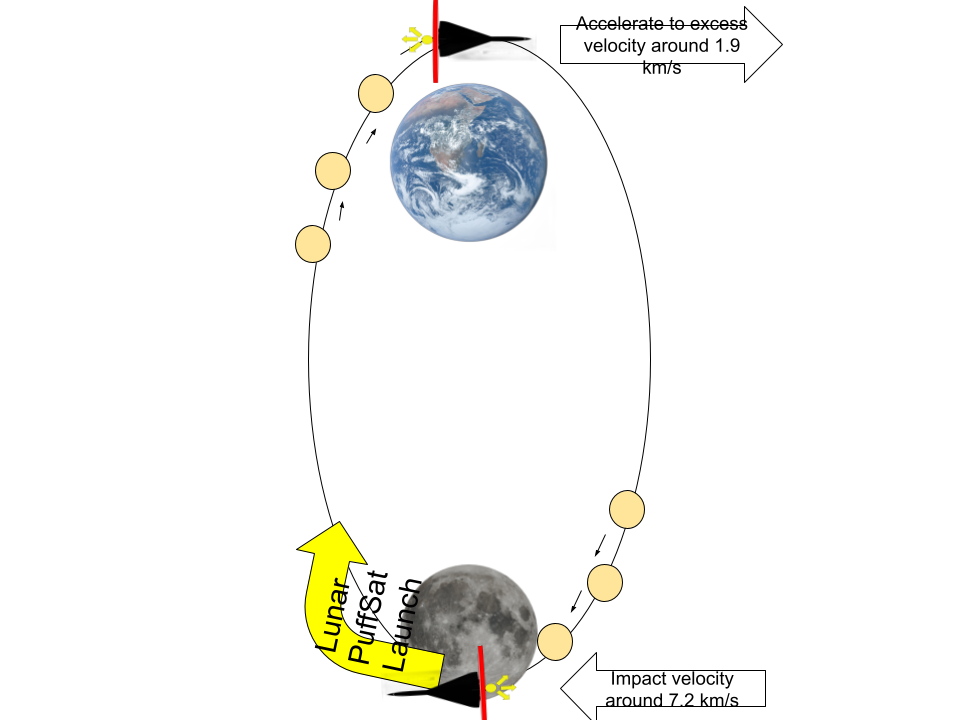
\includegraphics[width=0.5\linewidth]{images/Water Drawing From Moon.png}
    \caption{Lunar launched PuffSats replace Starship launched PuffSats \cite{earth_image} \cite{moon_image}}
    \label{fig:lunar_launched_PuffSats}
\end{figure}
Instead of using Starship, lunar volatiles extracted from the moon's permanently shadowed regions could fill our propulsive PuffSats. As shown in \autoref{fig:lunar_launched_PuffSats}, these PuffSats could be sent into a trans-lunar injection orbit that intersects our terrestrial suborbital rocket plane. Although PuffSat skins and electronics would likely still be sourced from Earth, volatiles constitute the majority of the PuffSats' mass. One approach to launching these PuffSats into orbit involves using rockets powered by lunar-derived propellants. The space community is enthusiastic about water electrolysis to produce and store cryogenic fuel for lunar rockets \cite{nasa_water}. However, this process is energy-intensive and requires complex cryogenic infrastructure, particularly for hydrogen fuel. Moreover, a reusable lunar rocket designed for repeated landings would require approximately \SI{6}{\km\per\second} of $\Delta V$, necessitating propellant mass fractions near 75\% for hydrogen or 80\% for methane. While these figures are an improvement over Earth-launched rockets, the high propellant mass fractions remain a significant challenge.   

\subsection{Lunar Rockets Without Lunar Rocket Fuel} \label{sec:lunar_rockets_no_fuel}
Instead of launching our lunar volatiles towards Earth with conventional rocket fuel, we launch off the moon using the same PuffSat pulsed propulsion we've been discussing for terrestrial launches.   A rocket launched with PuffSat pulsed propulsion from the lunar surface into a trans lunar injection orbit can burn its engines at periapsis around Earth.  Due to the Oberth effect, a small burn near Earth returns the rocket to the moon with a large velocity change.  As the rocket approaches the moon, it deploys its payload of PuffSats previously filled with lunar volatiles.  These returning PuffSats can push a new, more massive rocket filled with fresh volatiles off the moon.   We can then repeat this  cycle for exponential growth in lunar PuffSat launch mass capacity.   We've reduced combustible fuel requirements by burning our rockets near Earth.


\begin{table}[htpb!]
    \centering
    \begin{tabular}{|c|c|}
        \hline
        Before Collision & After Collision \\\hline
        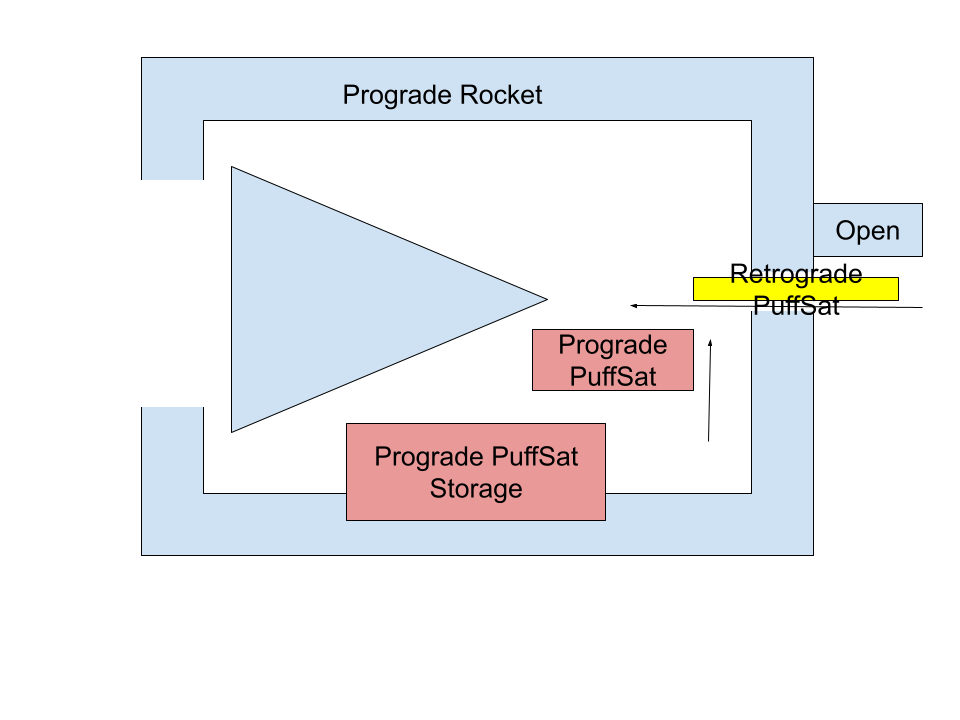
\includegraphics[width=0.45\textwidth]{images/Pulsed Propulsion Chamber Before Impact.png} &
        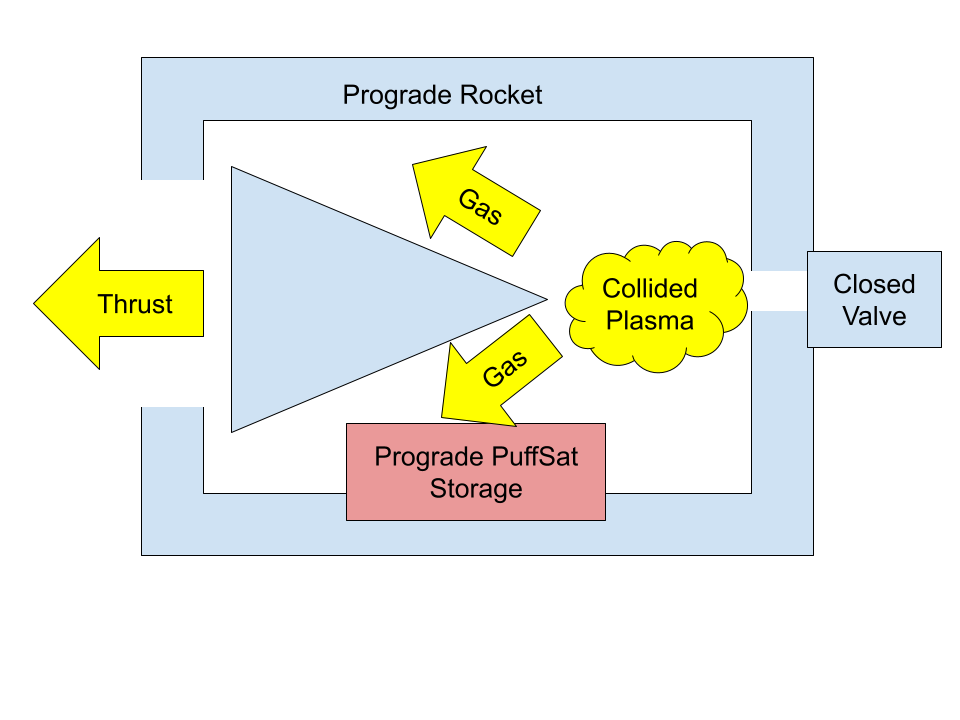
\includegraphics[width=0.45\textwidth]{images/_Pulsed Propulsion Chamber After Impact.png} \\ \hline
         
    \end{tabular}
    \caption{A pulsed propulsion chamber.   PuffSats enter, collide and produce thrust.   The valve, likely a fast rotating door synchronized with PuffSat arrivals, is optional because a small front opening will produce less thrust than a large rear opening.  If the explosion turns the gas into plasma, the valve could be magnetic rather than solid state.}
    \label{tab:pulsed_combustion_illustration}
\end{table}

However, we ideally don't want to make any chemical rocket fuel at all.   Let's again use PuffSat propulsion to launch our PuffSat deployment rocket from the lunar surface into a trans-lunar orbit.   We also launch a second set of PuffSats from the lunar surface into a retrograde trans-lunar orbit.   Using the centimeter precision navigation techniques we've discussed, we sequentially collide these retrograde PuffSats with more massive prograde PuffSats the main rocket is carrying.  As depicted in \autoref{tab:pulsed_combustion_illustration}, we trap the exploding gas from these collisions in a pulsed propulsion chamber and redirect this gas for thrust.   To leverage the Oberth effect and maximize gas collision velocity, we collide our PuffSats close to periapsis near Earth.

If our colliding PuffSats each travel at $v_p=\SI{11}{\kilo\meter\per\second}$, then from \autoref{eq:max_m_rp} derived in \autoref{sec:dv_effective},  the maximum theoretical combined effective exhaust velocity is $v_e = \frac{1}{2}v_p = \SI {5.5}{\kilo\meter\per\second}$.  Suppose this pulsed explosion has significant real world losses for an effective exhaust of $v_e = \SI{3}{\kilo\meter\per\second}$.   If the main rocket accelerates at its Earth periapsis with a burn of \SI{1.9}{\kilo\meter\per\second} it will reach the moon at \SI{7.2}{\kilo\meter\per\second} \cite{Katz_aim_is_all_you_need_2025}.   If the rocket deploys propulsion PuffSats on lunar approach, they can push another rocket off the moon with a mass greater than the incoming PuffSats. Specifically, the incoming propulsion PuffSats have enough momentum to start an exponential growth cycle where each loop around the moon launches about 1.455 times the starting mass.   If we do this once per lunar month, we have increased our initial launch mass capacity by a factor of 1 million in about 2.8 years \cite{Katz_aim_is_all_you_need_2025}. 

\subsection{Lunar Oxygen Has Mass And That Is All It Needs}\label{sec:lunar_mining}
Lunar volatiles like water ice are ideal for filling PuffSats, but they are scarce.   However, oxygen is very common in lunar surface minerals.   Using solar energy and mining rovers derived from platforms like the IPex Pilot Excavator \cite{ipex_pilot_excavator}, we can produce oxygen.  On the volatile-depleted sunlit lunar surface, finding something to burn oxygen with for rocket propulsion is hard.   However, PuffSat pulsed propulsion does not require oxygen combustion, just gas momentum.  In shadowed craters or artificial shade, lunar derived oxygen will liquify and perhaps even solidify for storage.  

We use some of our lunar PuffSats for pulsed propulsion to lift terrestrial suborbital supply rockets into low Earth orbit.  The supplies include solar panels, pusher plates, PuffSat skins, electronics, and rovers. These supply rockets then use conventional engines to gain \(\Delta V\) so they can resupply our lunar surface operations.   When they reach the moon, we also use PuffSat pulsed propulsion to decelerate for lunar landing.  The deceleration propulsion PuffSats would previously have been launched from the moon's surface into an eccentric lunar orbit opposite to the incoming supplies' velocity.   We can optionally reduce terrestrial resupply requirements by embracing basic lunar manufacturing using metals like iron that are byproducts of lunar oxygen production.  These lunar metals could be shaped into pusher plate and pulsed propulsion chamber components.  

We use the rest of our lunar PuffSats to exponentially grow our PuffSat mass capacity in orbit using the Oberth cycle discussed in \autoref{sec:lunar_rockets_no_fuel}.  Oxygen production is very energy intensive and lunar regolith will likely degrade machinery somewhat faster than equipment would degrade on Earth.  Nevertheless, regolith resistant machines  may still enable propulsion at costs that make hypersonic travel scalable.

\subsection{Jurassic Dark: Lunar Cold Trap Paleontology and PuffSat Mining Ethics}\label{sec:jurassic_dark}
In \autoref{sec:lunar_rockets_no_fuel}, we explored using lunar volatiles from permanently shadowed craters for PuffSat pulsed propulsion. These extremely cold craters could also indefinitely preserve DNA and other biomolecules from Earth impact ejecta \cite{dino_dna}. While speculative, the potential scientific value of lunar cold trap paleontology obligates us to check for frozen fossil biomarkers as we mine lunar ice for PuffSat propulsion.

We could analyze the volatiles we're extracting to see if they contain homochiral organic molecules, which are only produced by living organisms.   Studying samples that contain homochiral molecules would offer a unique window into Earth's entire biological history, potentially revealing how life began. And, of course, the discovery of dinosaur DNA would surely delight \textit{Jurassic Park} \cite{jurassic_park} fans.

\section{Sorry, I Don't Need ISRU}
\subsection{The Need For Speed} \label{sec:no_isru_rocket}\cite{topgun1986needforspeed}
If our propulsion PuffSats can reach high enough velocities, we could directly launch terrestrial payloads heavier than the PuffSats themselves.   This would eliminate the need for lunar ISRU. Repeatedly executing this launch cycle with ever larger (or more numerous) payloads would enable exponential growth in our launch capacity. Consider a rocket launched from Earth carrying pulsed propulsion payload.   We send $\frac{3}{4}$ our payload on a prograde trajectory with a solar periapsis similar to the Parker Space Probe and the remaining quarter on the opposing retrograde trajectory with the same Sun grazing periapsis.  These trajectories require high $\Delta V$ but we can use Jupiter gravity assists to achieve them (See \autoref{sec:jupiter_gravity_initial}).   These payloads release micro-thrust precision steered projectiles (see \autoref{sec:solid_PuffSats}) which then collide sequentially at periapsis in a pulsed propulsion chamber as described in \autoref{sec:dv_effective}. In propulsion chambers that minimize energy losses, the resulting plasma can produce effective exhaust velocities of \SI{100}{\kilo\meter\per\second} or higher, depending on periapsis. Perhaps we accelerate from \SI{200}{\kilo\meter\per\second} to \SI{250}{\kilo\meter\per\second} with Earth crossing speeds around \SI{150}{\kilo\meter\per\second} \cite{Katz_aim_is_all_you_need_2025}.  At these Earth crossing velocities, incoming PuffSats could collide with PuffSats aboard a new terrestrial rocket in the rocket's propulsion chamber.  With the thrust from these collisions, our payload would then be sent on prograde and retrograde orbits with low solar periapsis, repeating the cycle.  If desired, we can optimize exhaust velocity further by lowering the periapsis in steps, allowing our payload to fall significantly towards the Sun after each step.  This way, collisions after each periapsis reduction occur at progressively higher velocities for greater effective exhaust velocity.   If we double payload mass every 6 months, we increase our initial payload by a factor of 1 million in less than a decade \cite{Katz_aim_is_all_you_need_2025}. 

\subsection{Radiative Differences From Project Orion}\label{sec:radiative_differences}
Project Orion required shaped explosives to redirect plasma towards the pusher plate because 80\% of the bombs' energy became black body X-ray thermal radiation \cite{toughsf_cassaba_howitzer}.  In contrast, our proposed system anticipates minimal radiative losses from collisions, even at speeds matching the Parker Solar Probe. Though detailed computer analysis is needed for full confirmation, our reasoning for this low loss stems from
\begin{itemize}
    \item The colliding atoms in our system have a much lower atomic mass than fissile atoms. For a given total kinetic energy, this means the energy is distributed among a greater number of particles, resulting in a significantly lower average kinetic energy per particle, which directly translates to lower plasma temperatures. Additionally, plasmas formed from lighter elements generally have a higher specific heat capacity, meaning they absorb more energy for a given temperature increase. 
    \item The mean velocity of colliding atoms is likely about $\frac{1}{5}$ that of atoms in an inefficient 1\% yield bomb.  Since kinetic energy is proportional to the square of velocity, this alone suggests peak temperatures at least 25 times lower.
    \item Combined, lower mean velocity and atomic mass imply temperatures might be 200 times lower in our collision than in a bomb.  Radiative power rises with the fourth power of temperature ($T^4$), so peak radiation flux is likely around 1 billion times less than the least efficient nuclear bombs.
    \item The colliding masses should be much smaller than a nuclear bomb, with a lower radiative surface area.   As the collision plasma expands adiabatically, its volume increases proportionally faster relative to its initial volume compared to a larger bomb plasma for a given absolute linear expansion. This more rapid proportional change in volume leads to a quicker and more substantial decrease in temperature, further reducing radiative output.
\end{itemize}

Lower temperatures generate longer-wavelength blackbody X-rays compared to those from bombs. This means materials with lower atomic numbers (lower Z) can absorb this radiation and keep the plasma opaque. While Project Orion favored expensive and difficult to work with tungsten \cite{toughsf_cassaba_howitzer}, these longer wavelengths should allow for the use of cheaper elements to achieve plasma opacity.

\subsection{Solid Projectiles Rather Than Gas Generating PuffSats}\label{sec:solid_PuffSats}
Given the extreme velocities at periapsis, we no longer collide low density PuffSat produced gases because solid objects vaporize into opaque plasma.   Despite the harsh conditions, the corona's low perturbation environment (see \autoref{sec:periapsis_challenges}) enables high precision.  Like Proba-3, we aim to achieve the millimeter-scale precision critical for hitting small solids head on.   The real-world efficiency of these plasma explosions is likely high because the extreme temperatures and near-perfect targeting should bring the entire plasma to thermal equilibrium before significant expansion occurs.

We'd make these solid projectiles primarily from cheap low atomic number (low Z) materials like boron nitride, motor oil, and graphite.  A small amount of cheap higher Z materials like iron would be included to ensure opacity to the blackbody X-rays produced.  
All the projectile's mass contributes to propulsion, irrespective of its composition.  As shown in \autoref{fig:parker_cross_section}, the projectiles can contain electronics, heat shielding, and some liquid that passively or actively cools the skin through a centrifugally driven convection cycle.    When close to the Sun, they can operate on batteries or compact heat engines, like MEMS-scale Stirling engines \cite{mems_stirling_engine}. These alternatives are good options  where overwhelming solar saturation can diminish the performance of traditional photovoltaics.    

\begin{figure}
    \centering
    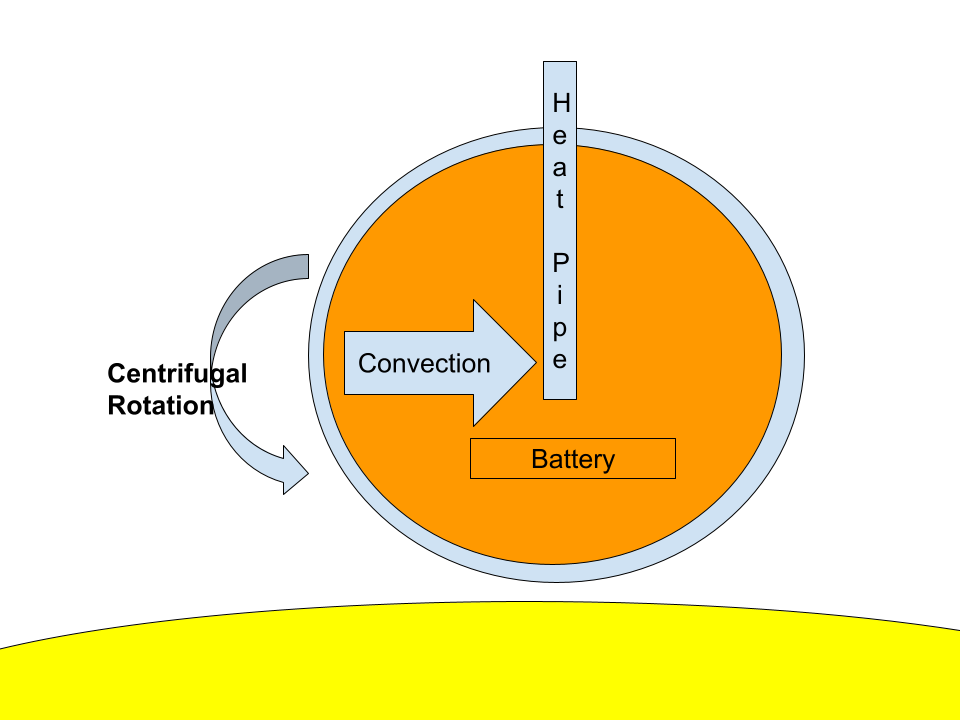
\includegraphics[width=0.5\linewidth]{images/Parker Projectile Cross Section.png}
    \caption{This cross-section shows a projectile with a highly reflective, heat-tolerant skin that is cooled by a centrifugally driven fluid. Heat is radiated away through a pipe that extends into the projectile's shadow, or at least to areas that receive sunlight obliquely. Batteries and electronics provide power.}
    \label{fig:parker_cross_section}
\end{figure}

\subsection{Navigation Challenges Near Periapsis}\label{sec:periapsis_challenges}
Close solar periapsis involves some unique challenges.   Obviously, any sensor dependent on visible light will need to filter interfering solar illumination.   Instruments will need to handle heat and solar wind.  Relativistic influences are predictable but must be included in trajectory calculations.  High collision speeds demand extremely accurate navigation.   The pulsed propulsion chamber may ablate slightly on each pulse.  The impacting projectiles must be miniaturized to at most a few kilograms to contain the immense energy from explosions at these velocities. The most significant problem is managing unpredictable changes in solar luminosity.  While average radiation pressure can be baked into our navigation, variations caused by sunspots and other magnetic phenomena complicate guidance prediction. Fortunately, recent research suggests that neural networks can improve weather predictions that influence luminosity and the coronal atmosphere \cite{lam2023learning}.  Despite the extreme environment, solar approaches to within the outer corona experience relatively mild total perturbations. Because the solar corona is so tenuous, the unpredictable effects of solar wind drag and gravitational variation are actually less severe than the perturbations experienced by satellites in low-Earth orbit \cite{leo_orbit_perturbation_simulation, corona_density}.  This low perturbation environment enables navigation precision beyond what we can achieve in low Earth orbit.
  
Spacing PuffSats sequentially far apart  may be hard.  Objects far apart at periapsis get closer together as radial distance grows.  As a result, Earth distance propulsion PuffSats would need to impart relatively high acceleration in short times.  However, the terrestrial payloads we're directly accelerating this way should be unmanned.   

When we lift high value payloads like astronauts into Low Earth Orbit, we use two sets of propulsive PuffSats. First, our Earth crossing PuffSats from the Sun push unmanned payloads into eccentric orbits around Earth. Then these eccentric payloads deploy PuffSats to push vital cargo like people or  satellites just as we discussed in \autoref{sec:starship_safelaunch}.

\subsection{Initial Periapsis Orbits With Jupiter Gravity Assists} \label{sec:jupiter_gravity_initial}
A final issue is placing the initial payload in a retrograde low periapsis solar orbit.  The best approach for this is likely using a gravity assist from Jupiter, which was the original plan for the Parker Space Probe mission \cite{mccomas2005solar}. 

To operate in deep space without relying on large solar arrays, the spacecraft may draw power from fuel cells or batteries. However, electrochemical systems are notoriously difficult to optimize under extreme cold. To mitigate thermal constraints, exothermic fuels can provide localized heating.  Alternatively, power can be generated via miniaturized chemically driven heat engines such as MEMS-scale gas turbines \cite{mems_gas_turbine}. If these energy sources utilize explosive reactants or yield volatile reactant products, these compounds can later be repurposed as PuffSat propellants---contributing to momentum transfer on impact. Near Jupiter, the PuffSats' volatiles would freeze and serve as effective radiation shielding. Together, the internal power source and shielding infrastructure would permit a close Jupiter flyby that maximizes our gravitational slingshot.

Optionally we can push more mass into the initial orbit by using a Jupiter gravity assist (possibly with a burn at Jupiter to leverage its Oberth effect) to place propulsion PuffSats into a retrograde Hohmann trajectory back to Earth.   They would cross Earth at around \SI{69}{\kilo\meter\per\second}, which could push a larger terrestrial payload onto  prograde and retrograde colliding trajectories at low solar periapsis.

\subsection{Jupiter-Only Exponential Launch Growth}\label{sec:jupiter_only_growth}
A simpler way to bootstrap an exponential launch cycle is to use the retrograde Hohmann trajectory from Jupiter described in \autoref{sec:jupiter_gravity_initial} but without close solar approaches.   PuffSats returning from Jupiter can push more than 9 times their weight into a highly eccentric orbit around Earth.   A small conventional burn coupled with solar electric engines and gravity assists with the inner planets can return this payload to Jupiter and restart the cycle.     The growth is slow compared to other proposals but may provide sufficient launch capacity to supply the satellite market within a few decades.

We can also combine this Jupiter launch cycle with reusable rockets or the lunar ice based cycle discussed in \autoref{sec:lunar_rockets_no_fuel}.  By increasing the number of initial PuffSat launches toward Jupiter, we can more rapidly scale up our launch throughput. Once this throughput is established, Earth based payloads can ride the returning PuffSats to orbit, enabling a sustainable and repeatable launch cycle.

\subsubsection{Venus and Mars Assist Alternatives}
PuffSats can employ gravity assists from Venus or Mars as alternatives to the Jupiter-only cycle. By using electric propulsion and deep-space maneuvers, these spacecraft can redirect their trajectories back to Earth at high velocities. Compared to Jupiter, inner-planet encounters occur more frequently and require significantly less $\Delta V$ to reach from Earth.   

Flybys of Venus and Mars yield much lower Earth-relative velocities---typically between \SI{10}{\kilo\meter\per\second} and \SI{20}{\kilo\meter\per\second}.  This is significantly less than the \SI{69}{\kilo\meter\per\second} return velocity from Jupiter. These lower velocities limit the payload multiplication achievable per cycle. However, the faster turnaround time of inner planet maneuvers can offset this limitation, resulting in total payload growth rates comparable to those of Jovian reverse Hohmann transfers. By strategically combining assists from Venus, Mars, and Jupiter, mission planners could modestly enhance overall throughput by increasing the frequency of favorable launch windows for PuffSat missions.

\section{One Hiroshima Per Second. The World Set Free}\label{sec:world_set_free}
In \autoref{sec:no_isru_rocket}, we propelled PuffSats to \SI{150}{\kilo\meter\per\second} at \SI{1}{\astronomicalunit} using solar gravity and pulsed propulsion. A \SI{60}{\tera\watt} pulsed heat source, which is equivalent to one Hiroshima bomb per second \cite{hiroshima}, requires harnessing the kinetic energy of just \SI{5.3}{\tonne\per\second} of propulsion mass at these speeds. For context, humanity's total power consumption is approximately \SI{20}{\tera\watt} \cite{owid-energy-production-consumption}. Given that typical power plants are roughly one-third efficient, a single one of these pulsed heat sources could meet the energy needs of all human civilization.  Remarkably, this concept evokes H.G. Wells's prophetic vision in his 1913 novel, \textit{The World Set Free}, where he imagined atomic bombs as a "blazing continual explosion" \cite{wells1914world}.  

Using kinetic projectiles to generate terrestrial power only makes sense if it achieves massive economies of scale that outperform the linear costs and land use efficiency of conventional renewables.  Let's explore how to build such a truly ambitious megastructure, and then explain why it's economically attractive in \autoref{sec:strawway_economics}.     

\subsection{Straw Ways To Heaven}\label{sec:straw_way_to_heaven}
The most common proposal for utilizing space-based power on Earth involves wireless power transfer from orbiting power plants to terrestrial rectenna arrays \cite{malaviya2022comprehensive}.  Unfortunately, long distance wireless transfer requires breakthroughs in wireless beam focusing \cite{space_beaming_power} and large radiators for dissipating heat. Moreover, the required wireless transmission infrastructure, both in space and on Earth, would be colossal.  Given these challenges, let's investigate terrestrial solutions that directly convert kinetic impact energy to electricity on Earth.

To deliver kinetic energy projectiles to Earth, the projectiles must be able to withstand atmospheric entry.  One solution is to build a vacuum tunnel, extending from Earth's surface to space, precisely aligned to allow incoming projectiles to pass through unimpeded.  The tunnel is suspended from an anchor point as depicted in \autoref{fig:straw_way_to_heaven}.   Enthusiasts have proposed numerous physically plausible structures that could support an anchor hoisted above Earth's atmosphere. These include Lofstrom Launch Loops \cite {lofstrom_loop}, tethered and global orbital rings, space elevators, and space fountains \cite{isaac_arthur_megastructure_complation}.  However, these ambitious ideas generally suffer from very low Technology Readiness Levels (TRLs), meaning they are far from practical implementation.

\begin{figure}[htpb]
    \centering
    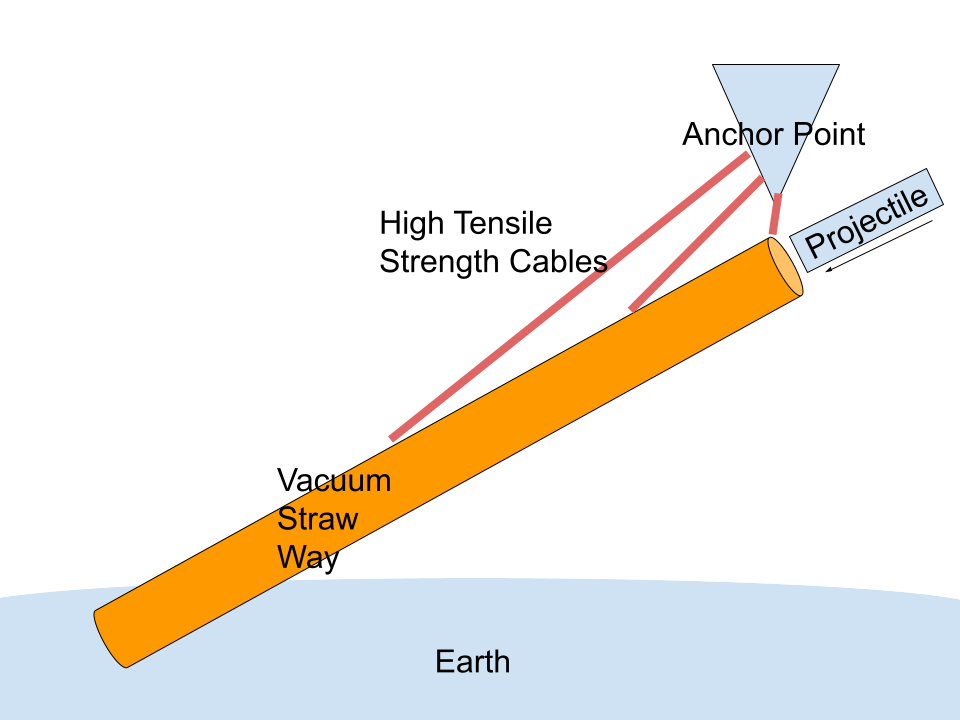
\includegraphics[width=0.5\linewidth]{images/Straw Way To Heaven.png}
    \caption{Vacuum tube suspended from cables allows projectiles through the atmosphere}
    \label{fig:straw_way_to_heaven}
\end{figure}


Fortunately, PuffSat pulsed propulsion offers a promising path to position an anchor point above Earth. While this technology also lacks significant technical maturity, we would have already developed it to highly reliable standards if we were using it to direct projectiles at Earth using the techniques from \autoref{sec:no_isru_rocket}}.  

A heavy-lift launch vehicle—such as SpaceX’s Super Heavy \cite{spacex_super_heavy}—delivers the anchor assembly and its attached vacuum tube to the target altitude.   We then indefinitely hover the anchor point using equal mass PuffSats that collide their gas output head-on in a pulsed propulsion chamber (described in \autoref{sec:lunar_rockets_no_fuel}), redirecting thrust downward. The propulsion chamber exhaust can be angled slightly to provide thrust vectoring to counter atmospheric winds on the vacuum tube and support cables. From this elevated anchor point, we sequentially deploy tube segments and support cables downward until reaching the ground. A reaction control system on the anchor point adjusts the pulsed propulsion chamber so it stays precisely positioned for the next PuffSat collision.  If these PuffSats meet at $v_p=\SI{11}{\kilo\meter\per\second}$ at an average mass flow rate of \SI{1}{\tonne\per\second}, they can theoretically suspend more than \SI{1100}{\tonne}.   

In reality, energy losses would reduce thrust.   For robust operations, we would need to lift redundant anchor points and vacuum tubes.  Together, redundancy and energy losses imply we will need additional PuffSat propulsion collision mass per second.  To keep the vacuum tube aloft, PuffSat propulsion must remain continuously active even when incoming projectiles cannot enter the tube to generate energy. Alternatively, for maintenance, the tube could be lowered at night and then re-hoisted by a heavy-lift rocket the following day.  Compared to magnetic systems like Lofstrom Launch Loops, hoisting an anchor with rockets or Puffsat pulsed propulsion is extremely energy inefficient. Nevertheless, lifting a few tons per second of propulsion PuffSat mass from Earth (as in \autoref{sec:starship_safelaunch}) or the moon (as in \autoref{sec:lunar_rockets_no_fuel}) seems economically viable if we use our vacuum tube to cleanly produce all the energy required by mankind. 

\subsection{Vacuum Tube Details}\label{sec:vacuum_tube_details}
To mitigate micrometeorite risk in the upper atmosphere, the vacuum tube incorporates sacrificial shielding or modular, swappable segments. Self-healing materials \cite{self_healing_material_survey} may repair small tube ruptures.  For example, a thin wire mesh embedded in the tube wall could detect conductivity changes caused by tears or punctures. Briefly increasing the current through these wires would cause localized heating, melting the surrounding material and heat-sealing small breaches. Redundant parallel tubes may also be deployed to ensure continuous operation despite localized damage.  

The tube's walls get thinner at higher altitudes, where less structural support is needed to maintain a vacuum.  At lower heights, ribbed or corrugated designs  keep the tube lightweight and flexible. Thin, high-strength tensile cables attached every few meters along the tube connect the tube and the anchor point.  Each attachment point includes several parallel tensile cables, ensuring structural redundancy in the event that one or more are severed by micrometeorite impacts.   Equipped with winching micro-actuators, these cables dynamically control their length to precisely tune the tube's curvature. The actuators shape the tube to counteract various forces---including Coriolis, tidal, and drag forces, as well as gravity changes---that affect the projectile's transit. The anchor point itself will rotate throughout the day to track the Sun.  Sensors along the vacuum tube measure and broadcast the tube's position and shape, allowing incoming projectiles to navigate through it accurately.

Additional sensors are placed along the cables and at the top of the tube to accurately measure any perturbations. These measurements help to precisely model the projectile's trajectory as it enters the tube. Once a projectile is inside, making adjustments with micro-thrusters would contaminate the vacuum and damage the walls. Instead, if the tube is metalized or partially conductive, we can steer projectiles using small magnets. These magnets generate Lorentz forces from induced currents in the walls, allowing for precise control.

Creating and maintaining a high vacuum in long tunnels is no simple task, but facilities like the Large Hadron Collider (LHC) prove it's feasible. Our tube, like the LHC's, uses non-evaporable getter (NEG) \cite{neg_coatings} thin-film coatings placed at intervals to chemically scavenge most atmospheric gases. These coatings, however, are ineffective against noble gases like argon. While we could embed cryopumps throughout the tube, that would introduce significant complexity and mass. Fortunately, when our projectiles collide with residual argon atoms, the atoms rebound at extreme velocities.  At these speeds, argon atoms become implanted a few nanometers deep into vacuum tube walls.  However, these impacts also sputter atoms from both the walls and the projectiles. The NEG coatings scavenge sputtered volatile atoms, while non-volatile elements recondense onto the tube interior.  Together, NEG coatings and argon implantation preserve vacuum integrity despite atomic sputtering. To ensure an even better vacuum inside the tube, thin films of oxygen-specific chemical adsorbents  are applied to the top few kilometers. By limiting exospheric oxygen from building up in the tube, we make our vacuum potentially even better than that of low orbit environments.  Scheduled tube refurbishment or replacement will be necessary due to wear from micrometeorites, argon sputtering, and NEG chemical consumption. Even if we pessimistically need a replacement once per month, the costs are minor compared to the revenue from global power generation.

Projectiles that catastrophically miss the vacuum tube cause only moderate Chelyabinsk-level \cite{popova2021chelyabinsk} ground effects because their extreme velocity guarantees they burn up at high altitudes.   Assuming our vacuum tubes are in remote areas, this causes minimal disturbances to population centers.   The vacuum tube itself is likely destroyed, but redundant vacuum tubes would then be moved into place.

\subsection{Tether Tapering And Countering Extreme Drag Forces}

Incoming projectiles experience dynamic pressure approximately  $\frac{v_{\text{projectile}}^2}{v_{\text{PuffSat}}^2} = \frac{(150\,\text{km/s})^2}{(11\,\text{km/s})^2} \approx 185$ times greater than that faced by trans-lunar PuffSats, due to their much higher velocity. This amplifies drag forces far beyond those analyzed in \autoref{sec:estimate_cold_gas}.

Because these projectiles spend only \SIrange{1}{2}{\second} at lower altitudes when arriving at such extreme velocities, we may be able to counteract the resulting terminal forces by briefly firing small chemical thrusters and vectoring their thrust. Despite the rarefied air at \SI{200}{\kilo\meter} altitude, projectiles still face intense ram heating. Thin, thermally conductive skins can be cooled via convective heat transfer and latent heat absorption from phase-changing PuffSat volatiles (e.g., water vaporization).

Projectile guidance and thermal management are significantly easier if projectiles enter the vacuum tube at \SIrange{300}{400}{\kilo\meter} altitude, rather than the \SI{200}{\kilo\meter} baseline used in \autoref{sec:formation_challenges_current_missions}. These higher altitudes slightly exceed the breaking length of commercially available materials like Kevlar or SK99 Dyneema (modified with carbon for creep resistance) \cite{wiki:specific_strength, sk99_tension}.

Unlike the projectiles, PuffSats that provide pulsed propulsion to anchor the tube travel at only \SI{11}{\kilo\meter\per\second}. Their lower velocity enables more precise navigation and impact targeting at reduced altitudes. Therefore, we can place one anchor at the lower \SI{200}{\kilo\meter} altitude and connect the upper portion of the tube to a second anchor at higher altitude. Shorter cables anchored to surface vessels can serve as guy wires to counter winds on the lower \SI{20}{\kilo\meter} of the tube. These guy wires can be actively winched to adjust tension, minimizing peak wind forces the longer anchor cables must withstand.

Despite these optimizations, our current cable designs still lack sufficient engineering safety margin. Tapered cables offer a promising solution. The mass-optimal cross-sectional area of a tapered cable at distance $x$ from the anchor scales as $A(x) = C e^{-\frac{x}{b}}$, where $b$ is the material’s breaking length and $C$ is a constant (see \autoref{sec:breaking_length_derived}). 

To maintain an engineering safety factor of 3 across a cable stretched to its full breaking length, the cross-sectional area at the anchor must be roughly 20 times greater than at the point where the cable connects to the lowest portions of the tube. Fortunately, this tapering requirement aligns with our existing structural strategy: we already deploy thin control wires every few meters along the tube. By progressively merging and intertwining these wires near anchor altitudes, we achieve the required cross-sectional increase without adding significant mass beyond our existing budget.



\subsection{Power Plant Chamber Details}
Beneath the vacuum tube, we propose excavating a massive steam chamber designed to vaporize incoming projectiles. These chambers would be substantial construction projects, engineered to withstand sudden changes in pressure and temperature.  The chamber walls would be lined  with steel backed by bunker-grade reinforced concrete, while internally mounted spring-loaded metal plates would absorb shock and mitigate structural stress.  

Suppose a \SI{0.1}{\cubic\kilo\meter} steam chamber containing \SI{50}{\kilo\gram\per\cubic\meter} steam receives a \SI{600}{\tera\joule} kinetic impact.   As a simplification, let's say the steam has a constant specific heat of \SI{3.5}{\kilo\joule\per(\kilo\gram\celsius)}.  In this case the temperature change is 
$\frac{\SI{600}{\tera\joule}}{\SI{5e9}{\kilo\gram}\times\SI{3500}{\joule\per(\kilo\gram\kelvin)}} = \SI{34.2}{\celsius}$.  An impact of this magnitude every 10 seconds produces the heat to continuously provide all humanity's energy.  This steam chamber would be connected to thousands of turbines and a massive cooling loop to harness and dissipate this energy.  

Releasing large amounts of heat into the atmosphere would lead to unacceptable local temperature increases. Using a coolant loop that exchanges heat with deep ocean water will also have environmental consequences. Spreading $\SI{40}{\tera\watt}$ of heat over $\SI{10}{\cubic\kilo\meter}$ of deep ocean water would increase its temperature by $\frac{\SI{40}{\tera\watt}\cdot\SI{3600}{\second\per\hour}}{\SI{1e13}{\kilo\gram}\cdot\SI{4186}{\joule\per\kilo\gram\per\celsius}} = \SI{3.44}{\celsius\per\hour}$.  This rapid temperature change could severely damage local marine habitats.

However, considering the limited marine life found far above the ocean floor and below the sunlit zone, the broader deep sea ecology beyond the directly heated zone would remain stable. When compared to the widespread impacts of global anthropogenic climate change or even the significant displacement of wildlife from building solar farms, the environmental harm from this specific heat rejection method appears relatively modest.

The projectiles would have explosive or water interiors that disintegrate quickly on hypervelocity shock contact with the chamber's high pressure steam. Made from carbon composites and polymers, their structural exteriors would vaporize into gases at impact temperatures. Inside the steam chamber, temperatures are so high that the carbon turns into a superheated plasma. Steam also decomposes in these conditions, releasing oxygen that combusts this carbon along with any air present. Although this process forms very little carbon soot before the carbon turns to carbon dioxide, any that does form can be filtered out with charcoal screens before reaching the turbines.   The remaining gases are released or sequestered as they travel along with the steam cycling through the system.   Solid residues that precipitate on chamber walls could be cleaned off either continuously or during maintenance windows.  Continuous processes might rely on trapping solids in cheap viscous liquids like silicone fluids, organic oils, or molten salts that slowly ooze down chamber walls and drain at the bottom.  

\subsection{Vacuum Exchange And Airlock Details}\label{sec:vacuum_airlock}
An airlock separates the steam chamber from the rest of the tunnel as shown in \autoref{fig:power_plant_vacuum_exchange}.   A door with a closing speed of \SI{300}{\meter\per\second} could close a \SI{30}{\centi\meter} diameter aperture in \SI{1}{\milli\second}.  Even a \SI{5}{\meter} long airlock is long enough to prevent steam molecules from traversing the airlock in this short time.  

\begin{figure}[htpb]
    \centering
    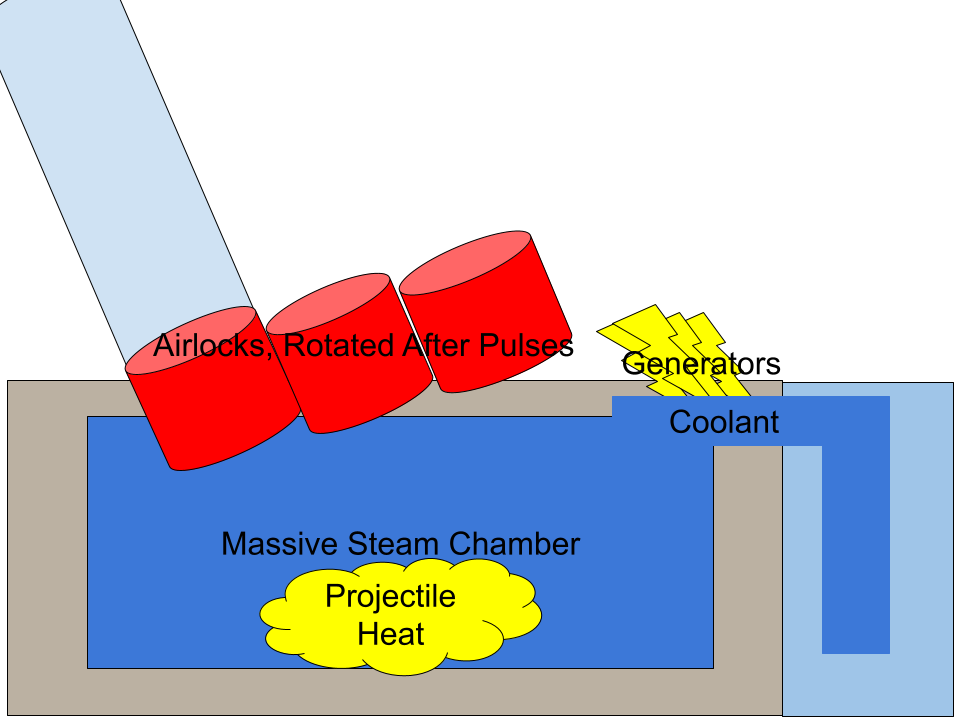
\includegraphics[width=0.5\linewidth]{images/Power Plant Cooling and Generators.png}
    \caption{Diagram of the power plant and vacuum airlock system; new airlock segments are rotated in between impacts.}
    \label{fig:power_plant_vacuum_exchange}
\end{figure}

Designing an airtight door that can open and close at the necessary speeds is beyond current technology. However, a system of rapidly rotating disks with strategically placed apertures can create a quick-closing, leaky seal.

This system works like this:

\begin{itemize}
\item Two or more pressure-resistant disks with identical radii of perhaps \SI{10}{\meter} are closely mounted on an axial shaft.

\item These disks spin at slightly different speeds, and each has a \SI{30}{\centi\meter} aperture near their outer edge.

\item We add mass along the radial line of each disk's aperture to keep the rotating disks balanced

\item When the apertures don't overlap, they block the vacuum tube and prevent steam from entering.

\item The apertures align every few seconds over the airlock opening.   This gives us time to close a second air-tight door over the airlock opening. 

\item The disk apertures may align more frequently than projectile arrivals.  Since arrivals might only arrive every \SI{10}{\second}, it's tricky to design fast spinning disks that only overlap at this low frequency.  As long as the secondary door can close between alignments, and the alignments are synchronized with projectile arrivals, the airlock system meets its operational requirements.
\end{itemize}

This rotating disk system offloads handling the pressure differential between steam and vacuum.  That simplifies the design for the separate, high-performance airtight door that seals the vacuum completely. The air-tight door is still fast, closing on the order of a few hundred milliseconds.  Before this door closes, steam leaks through the clearance between the disks and the airlock.  This clearance is likely at least a millimeter since we must handle vibrations.  To further mitigate steam ingress, chemical desiccants are embedded in the disk housing and airlock walls. Thin films of desiccants are also used along the first kilometer or so of the vacuum tube.  The disk housing and airlock walls might also be cooled to freeze or at least slow steam atoms.

At the bottom of the airlock, the projectile releases enormous heat on contact with steam. Asteroid air-burst simulations suggest the vast majority of this energy is directed in the projectile's direction of travel, away from the airlock and the closest chamber walls \cite{tunguska_downwards}. If still needed to handle the high initial heat, sacrificial plastic segments can form the bottom part of the airlock pipe. These plastics should be strong at low temperatures but vaporize easily to avoid creating shrapnel. Their brief exposure to steam before projectile impact can be buffered by a coat of ice, which forestalls heating. To prevent the production of highly toxic gases when they decompose, the plastic should not be halogenated. Cheap polyethylene pipes may satisfy all these requirements.  The pipe can be ribbed for strength and corrugated to stop buckling under the steam's pressure.  These techniques reduce the pipe mass needed to withstand the steam's compressive load.  A thicker plastic plug at the bottom of the pipe could drastically quicken projectile disintegration, especially if the projectile primarily contains materials like water or explosives. The enormous kinetic energy from the projectile's velocity would pulverize the projectile on plug impact. The resulting intense heat and shock wave breaks any solid debris into smaller shards that rapidly vaporize in the steam far from chamber walls.  An added benefit of these sacrificial segments is that they lengthen the time the airlock door has to seal before steam can travel far enough to enter the vacuum tube.

A new airlock segment is swapped in between kinetic projectile impacts, providing time to restore the high vacuum offline before its next use. Sacrificial bottom sections are also replaced and reattached while the main airlock segment is out of rotation.

\subsection{With Economies Of Scale, Our Ambitions Can Scale Too}\label{sec:strawway_economics}

While a global power plant requires a massive initial capital investment, its costs scale favorably with output. The cost of suspending a large vacuum tube depends very little on the plant's generating capacity. The cost of deep sea cooling loops would also be amortized across the entire planetary scale facility.  A multi-terawatt installation could achieve significant per-watt cost reductions through bulk procurement of thousands of identical turbine and generator units. 

Mass production reduces the cost of projectile electronics and micro thrusters. The cost of these components per projectile also remains nearly the same as individual projectile size increases.  Ten seconds of planetary scale power corresponds to $\SI{20}{\tera\watt} \times \SI{10}{\second} \approx \SI{5.56e7}{\kilo\watt\hour} = \$555,556$ at 1 cent per kilowatt-hour.  This energy cost would likely dwarf the material costs of the projectiles themselves, especially if their interiors are mostly water or explosives.      

Power from our plant could be globally distributed by supertanker-sized batteries that connect to urban power grids at coastal ports.  While the cost of utility-scale batteries is progressively declining, it remains a significant hurdle. Current battery designs prioritize efficient energy storage and release. However, if energy efficiency becomes less critical, we could design cheaper low performance batteries. Given that our power source exhibits strong cost efficiencies, we could simply increase the power output to compensate for any energy losses incurred by using these more affordable batteries for distribution. 

Fossil fuels remain entrenched as the dominant energy source, even as cleaner alternatives like batteries gain traction. High-temperature heat from low-cost projectile impacts offers a novel route for synthesizing hydrocarbon fuels directly from water and carbon dioxide.

One promising pathway is the cerium oxide cycle \cite{CeriaThermoCycles}, where cerium oxide is reduced at high temperatures and low pressures. Operating at low pressures simplifies vacuum chamber and airlock design (see \autoref{sec:vacuum_tube_details}). The reduced cerium oxide then reacts with carbon dioxide and water to produce carbon monoxide and hydrogen---precursors for hydrocarbon synthesis via industrially mature chemical processes \cite{water_gas_shift}.

An alternative approach, adapted from chemical looping in blast furnaces \cite{iron_chemical_looping}, uses iron to reduce carbon dioxide to carbon monoxide. This carbon monoxide can then be combined with water to produce fuels through standard chemical pathways \cite{fischer_tropsch}. The resulting iron oxide may be thermally decomposed to regenerate iron, forming a closed-loop cycle. Iron, being denser than iron oxide, naturally separates under gravity---much like the stratification of slag and molten iron during steel production. This gravitational sorting enables passive separation within the molten environment. Incoming projectiles can be designed to gasify just prior to impact, allowing energy deposition without direct mechanical disruption. At velocities around \SI{150}{\kilo\meter\per\second}, low-density gas atoms penetrate a few nanometers into the lava, transferring heat through shallow kinetic interactions. This reduces shock propagation and ejecta formation. To further enhance coupling, finely divided iron oxide powder can be injected into the vacuum chamber, presenting a much larger effective surface area to the incoming hot gas. The powder acts as a thermal sponge, absorbing and redistributing energy before it settles back into the molten pool. The chamber walls remain protected from peak loads by the intervening lava, which serves as both a volumetric heat sink and a radiative buffer, damping transient spikes.

Both cerium and iron oxides decompose only under very low pressures, requiring aggressive removal of oxygen from the reaction environment. An alternative approach is to use water splitting  cycles, such as the sulfur–iodine or copper–chlorine processes, to generate hydrogen \cite{sulfur_iodine_chlorine}. Hydrogen, together with carbon dioxide, forms an ideal feedstock for hydrocarbon synthesis. Although these water-splitting cycles typically operate at relatively moderate temperatures, they expose reactor walls to highly corrosive intermediates such as hot sulfuric acid. Modern ceramic matrix composite liners \cite{flexible_ceramic_composites} may provide the necessary combination of fracture toughness, corrosion resistance, and shock tolerance to enable practical thermal water-splitting systems.  These liners could coat a shock-absorbing nickel superalloy chamber \cite{inconel_718_strong}, which is externally heated by a molten bath of lava or liquid iron.  Projectile impact energy keeps the lava molten, indirectly providing the steady high temperatures that are optimal for the reaction chamber. This configuration also shields the ceramics from direct impact shocks. 

By bypassing costly steam turbines and simplifying vacuum tube maintenance, this direct-heating approach could enable viable hydrocarbon synthesis before large-scale electricity generation becomes cost effective.

Though the power plant and distribution infrastructure would cost billions to construct and operate, the revenue generated is staggering. Ultimately, we'd spend billions to make trillions annually from a planetary-scale plant.  Turns out, if  \textit{Superman} wants to be as rich as \textit{Lex Luthor}, he should get limitless energy not from the light of a yellow sun, but from its gravity \cite{superman2025}.

\subsection{Comparison To Project PACER}
Project PACER was a 1970s Los Alamos concept to generate power by extracting steam from nuclear bombs detonated in a salt cavern \cite{pacer_1975}.   Later improvements protected the cavern walls with an artificial waterfall of tritium breeding liquid salts \cite{pacer_revisited}.  

Unlike PACER, our proposal does not produce radioactive waste or encourage the mass production of nuclear weapons.   Should a liquid wall be needed to protect the chamber, it can be made from cheap materials like water.  Tritium breeding and extraction are not required.   Most critically, our design eliminates the need for a biological shield, simplifying the direct coupling of steam to turbines. This direct steam cycle enables the rapid heat exchange with the environment necessary to build terawatt-scale power plants.

\subsection{To Solve Climate Change, Make The Earth A \textit{Death Star}}\label{sec:death_star}
A \textit{Death Star} \cite{death_star} is a giant sphere with a  narrow 1 meter opening where you can shoot something down to create an explosion inside the main reactor.   Building a \textit{Death Star} from scratch  would be a huge undertaking.   Fortunately, if we build the Straw Way To Heaven described in \autoref{sec:straw_way_to_heaven}, we're living on one.  Although our Straw Way generator produces clean energy from incoming projectiles, its power production is restricted to daytime hours when the straw can face the sun.   Also, a limitless clean energy source would only slow climate change.   Industrial carbon emissions from steel, cement, agriculture, and other processes would still heat the planet \cite{steel_and_cement}.   

\subsubsection{That's No Moon .  Oh Wait, It's Literally Our Moon}\cite{kenobi1977moon}
Projectiles made from lunar materials could enter a terrestrial Straw Way from high angles of attack around the clock.  To generate \SI{60}{\tera\watt} of heat from lunar bombardment, we'd need an astonishing \SI{1}{\kilo\tonne\per\second} of lunar mass to pass through the terrestrial vacuum tube. Such a vast quantity is daunting, but the momentum for launching off the moon could come from kinetic projectiles inbound from the Sun (as described in \autoref{sec:no_isru_rocket}). Beyond providing thrust, these projectiles aimed at the Moon could vaporize lunar regolith. The resulting thermal energy could be harnessed for electricity generation or to power chemical and industrial processes directly. This lunar power source could support large scale mining and production of the oxygen gas used in PuffSat pulsed propulsion  (as discussed in \autoref{sec:lunar_mining}).

Lunar regolith is primarily carbon-depleted rock \cite{mckay1991lunar}. After the regolith-derived impactors heat steam to drive a global-scale generator, the process yields a waste column of hot regolith and scalding water. If this waste is channeled through thermally insulated pipes into deep ocean water, the intense hydrostatic pressure compresses the regolith. Its large surface area and elevated temperature accelerate chemical reactions that convert silicates into carbonates, pulling dissolved carbon dioxide from seawater. Deep ocean pressure further shifts chemical equilibrium toward carbonate formation. With an incoming regolith flow of $\SI{1}{\kilo\tonne\per\second} \approx \SI{31}{\giga\tonne\per\year}$, we could mineralize billions of tons of dissolved carbon dioxide annually. This would enhance the ocean’s capacity to absorb atmospheric carbon dioxide, making lunar mineral sequestration a viable strategy to offset most of the world’s industrial carbon emissions.



\subsection{Fusion Propulsion And Epstein Drives}\label{sec:epstein_drives}
The fast projectiles from \autoref{sec:no_isru_rocket} could propel a spacecraft around the inner solar system at relatively high speeds.   As our technology advances, we'd want to travel on brachistochrone trajectories under constant Earth gravity acceleration between the planets as envisioned in \textit{The Expanse} \cite{Corey2012Drive}.  Evaporative cooling and advanced heat shields like NASA's yttrium oxide based "solar white" might  enable spacecraft to approach the Sun to 2 solar radii \cite{ted_ed_2025_how_close}.  At this close solar periapsis, prograde and retrograde projectile collision velocities would exceed \SI{869}{\kilo\meter\per\second} \cite{Katz_aim_is_all_you_need_2025} in the reference frame of a fusion pulsed propulsion chamber on the target rocket.  

\begin{figure}[htpb]
    \centering
    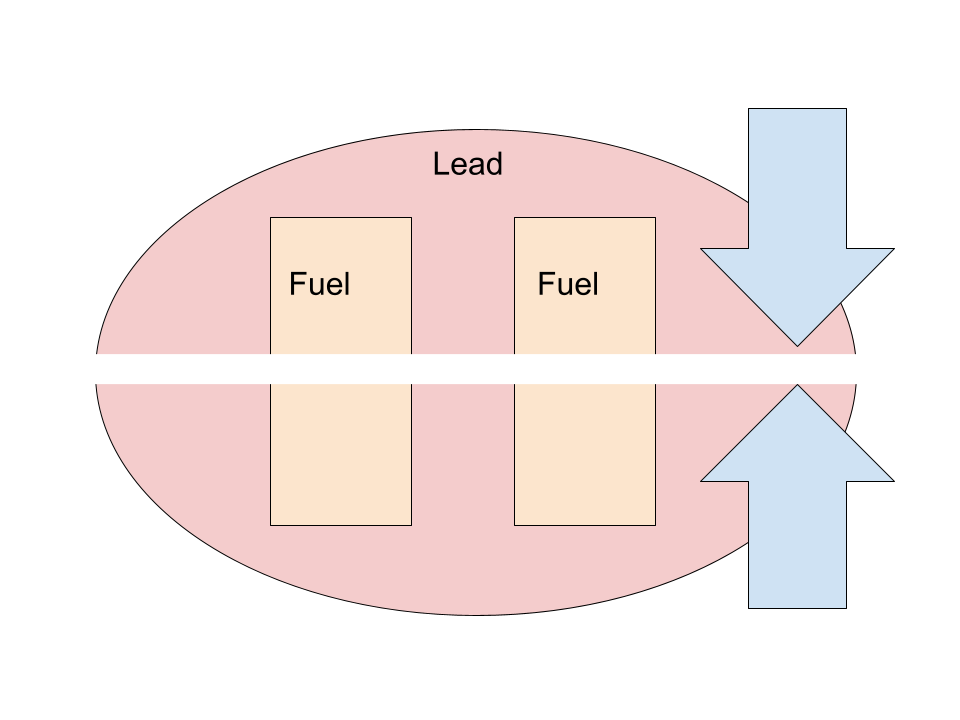
\includegraphics[width=0.5\linewidth]{images/Fusion Impactors.png}
    \caption{A lead tamper generates immense shock heating around fusion fuel and compresses it to ignition conditions during head-on collisions.  Lead embedded in the fuel also serves as a superheated Teller-Ulam style spark plug \cite{WikipediaThermonuclearWeapon} for fusion.}
    \label{fig:fusion_tamper}
\end{figure}

A 1979 Los Alamos Impact Fusion workshop concluded speeds of just \SI{200}{\kilo\meter\per\second} might be sufficient for precompressed gram sized fusion fuel projectiles to ignite \cite{impactfusion1979}.   Larger projectiles would likely be easier to confine long enough for high fusion energy gain.   A lead tamper, as depicted in \autoref{fig:fusion_tamper} surrounding a few hundred grams of fusion fuel could ignite fusion explosions and trigger immense exhaust velocities.  Shocked lead would reach even higher temperatures than the fuel because its high atomic number implies greater energy per atom (see \autoref{sec:radiative_differences}).  Therefore, lead or another high-Z material is centrally embedded in the fusion fuel at the tip of the colliding masses. This embedded lead serves as a "spark plug" for fusion, analogous to the secondary fission bomb in Teller-Ulam style \cite{WikipediaThermonuclearWeapon} nuclear explosions. Pulsed fusion propulsion would likely employ the shaped nuclear charges Project Orion explored to redirect energy and thrust.  
With mostly aneutronic fusion fuel, projectiles could reach velocities on the order of thousands of kilometers per second.  This is because aneutronic fusion directly converts energy into charged particle kinetic energy, bypassing the mass penalty of neutron shielding.  A seed of deuterium-tritium could ignite a larger deuterium and helium-3 mixture to achieve aneutronic fusion rocket speeds.   As the spacecraft accelerates, it can also reach speeds where it triggers fusion by crashing into slower moving fusion fuel targets.   If carefully planned, these chains of fast-moving projectiles could essentially create interplanetary highways, allowing people to travel between planets under comfortable artificial Earth gravity in time frames comparable to ocean liners crossing the Atlantic.  

\subsection{The Sixth Question For Climate Change}\label{sec:sith_question}
Bill Gates' excellent book, \textit{How to Avoid a Climate Disaster} \cite{gates2021avoid}, details five practical questions \cite{breakthroughenergy_2021_five} any effective climate solution must address. Our Straw Way To Heaven (see \autoref{sec:straw_way_to_heaven}) addresses Gates' questions better than other alternatives. It completely negates carbon emissions, reverses cement emissions, provides indefinite global power, occupies minimal space, and boasts marginal costs that decline rapidly with output.

Yet, I respectfully propose a sixth question that could galvanize the public to enthusiastically support a particular climate solution. Beyond just reducing our electric bills and helping the environment, how will this breakthrough drastically improve daily life? An investment on the scale required to solve climate change should ideally grant human society new abilities, such as hypervelocity transport and affordable space travel. PuffSat pulsed propulsion can achieve all of these things.  

\section{When We Get Greedy, We'll Go to Phoebe}\label{sec:greedy_phoebe}
In \autoref{sec:no_isru_rocket} we discussed using Sun-grazing Oberth maneuvers to accelerate projectiles to \SI{150}{\kilo\meter\per\second} at \SI{1}{\astronomicalunit}. These high velocities enable the large $\Delta V$ required to place the next suborbital rocket into prograde and retrograde colliding orbits near the Sun.  However, as detailed in \autoref{sec:periapsis_challenges}, such close solar approaches introduce severe engineering and operational challenges---potentially increasing projectile costs compared to less extreme solar encounters.  Additionally, suborbital rockets used to launch from Earth might produce unacceptable levels of pollution in the upper atmosphere.

Orbits with higher apoapsis require less $\Delta V$ to shed orbital angular momentum and lower their periapsis. For example, transferring to a solar impact trajectory from Saturn requires only about \SI{10}{\kilo\meter\per\second}, compared to roughly \SI{30}{\kilo\meter\per\second} from Earth. This makes Saturn a more efficient departure point for reaching the inner solar system or the Sun.

Saturn’s irregular moon Phoebe lies just $\SI{180}{\degree} - \SI{173.4}{\degree} = \SI{6.6}{\degree}$ from the solar ecliptic \cite{phoebe}, giving it a favorable alignment for interplanetary transfers. Its high altitude orbit around Saturn yields a low orbital velocity, enabling efficient low $\Delta V$ transfers to elliptical trajectories that match Phoebe’s apoapsis and dip toward Saturn at periapsis.  From Phoebe, a prograde rocket could be launched to collide with retrograde payloads also originating from Phoebe. These collisions could take place in a pulsed propulsion chamber near Saturn, enabling highly efficient Oberth maneuvers. With careful targeting to avoid Saturn’s rings, this method could launch spacecraft toward the inner solar system. Precisely aiming such collisions near Saturn is challenging, but likely easier than attempting similar maneuvers at the extreme conditions of close solar periapsis described in \autoref{sec:no_isru_rocket}. PuffSats launched from Saturn toward Earth could power a Straw Way generator (see \autoref{sec:straw_way_to_heaven}) or deliver suborbital rockets into orbit (see \autoref{sec:starship_safelaunch}).

These rockets could also return to Phoebe at high speeds, launching additional mass toward Saturn via pulsed propulsion. This bootstrapped launch cycle from Phoebe mirrors the lunar exponential growth loop discussed in \autoref{sec:lunar_rockets_no_fuel}, but benefits both from Phoebe’s lower escape velocity and from Saturn's larger gravitational Oberth effect. Power for mining operations on Phoebe could come from solar energy concentrated using lenses made from Phoebe's native ice or locally produced plastic. Fission reactors transported from Earth are another possibility, as is thermal energy generated by returning impactors.  One key advantage kinetic impact energy offers is that its power doesn't decline quadratically with solar distance—unlike solar panels.

With an estimated composition of nearly 50\% ice by mass \cite{phoebe}, Phoebe offers essentially unlimited volatile resources to fill PuffSats. Unlike the Moon’s permanently shadowed ice deposits, Phoebe’s ice-rich regions receive direct sunlight. Although faint, this illumination enables solar concentrators to generate power directly adjacent to mining operations. Phoebe’s abundant water could be used to wash regolith from equipment, mitigating the mechanical fouling that plagues lunar hardware. In addition, Phoebe’s regolith—composed largely of frozen volatiles—is likely softer and less abrasive than the Moon’s harsh dust, reducing wear on machinery. By contrast, lunar volatiles are scarce, and oxygen extraction from lunar regolith (see \autoref{sec:lunar_mining}) is highly energy-intensive.

Phoebe’s ultra-low gravity makes it difficult to anchor mining infrastructure securely. However, its volatile-rich composition allows a supplemental solution: retro-rockets powered by in-situ steam or chemical propellants manufactured from Phoebe's volatiles. To save energy, icy reaction mass could also be launched mechanically from Phoebe’s surface without first converting it to steam. If Phoebe’s gravity proves too low for certain operations, Iapetus could serve as a potential backup site. Similarly, Jupiter’s moon Himalia may support analogous maneuvers if exploration reveals significant volatile deposits.

Mining moons like Phoebe to supply PuffSat payloads is easier than extracting conventional raw materials for Earth delivery. PuffSats execute high-velocity flybys, eliminating the need for costly deceleration maneuvers or bulky reentry shielding near Earth. And unlike ice or gold, the ultra-high-energy-density pulses generated by PuffSat impacts are not just valuable—they’re irreplicable. No known terrestrial technology, short of nuclear weapons, can produce such large-scale high-density energy bursts.

\subsection{Mining Helium-3} \label{sec:mining_helium_3}
Helium-3 for aneutronic fusion may be available on the Earth's moon \cite{esa_helium3_mining}, but likely not in quantities to support large scale fast interplanetary transport like discussed in \autoref{sec:epstein_drives}.   However, the gas giants contain inexhaustible supplies of helium-3 \cite{palaszewski2005atmospheric}.   A nuclear fission thermal rocket or scram jet could extract helium-3 and hydrogen while flying in Saturn's atmosphere and then jump a few thousand kilometers above the atmosphere.  It could then separate from a payload carrying mined helium-3, falling back to Saturn to mine more.  An accident on such a fission rocket would cause no harm, because waste would simply fall into Saturn's core. Propulsion PuffSats from Phoebe could then send the helium-3 payload into the inner solar system for use in fusion rockets.  

If fission rockets prove politically unpalatable, chemical rockets may also work.   Chemical rocket fuel powers a motor in Saturn's atmosphere for the energy to mine helium-3.  The rocket then fires its rockets to hop above Saturn's atmosphere.   Propulsion PuffSats from Phoebe push the rocket into a stable orbit where it is refueled and releases its helium-3 payload.  Then new propulsion rockets decelerate the refueled rocket so that it falls into Saturn's atmosphere for another mining round.

\subsection{A Ceres-ly Good Alternative}\label{sec:ceresly_good}
Ceres may offer a Goldilocks environment for sourcing PuffSat materials. The Dawn mission revealed that up to one-third of Ceres' mass could be water ice \cite{ceres_ice}, accessible within \SI{1}{\meter} of the surface at high latitudes. Near-surface deposits may also contain nearly 20\% carbon \cite{ceres_carbon_nitrogen}, enabling in-situ production of methane and other volatiles. Additionally, nitrogen-rich phyllosilicates found on Ceres are promising for fabricating micro-explosives \cite{ceres_carbon_nitrogen}. In short, Ceres contains all the essential chemistry for manufacturing icy PuffSats on-site (see \autoref{sec:icy_puffsat}).

Operationally, Ceres offers several advantages: adequate solar illumination for power generation, just enough gravity to support mining infrastructure, shorter transit times than Phoebe, and a low escape velocity. A solar impact trajectory from Ceres requires only about \SI{18}{\kilo\meter\per\second}, significantly less than from Earth. This lower $\Delta V$ supports Ceres-based launch cycles that harness the Oberth effect near the Sun with less extreme perihelion or increased payload capacity per cycle relative to Earth-based alternatives (see \autoref{sec:no_isru_rocket}).

Achieving centimeter-accuracy PuffSat interceptions around Ceres may prove easier than in most other prime solar system locations. In high-altitude, easily accessible orbits above Ceres, PuffSats would encounter negligible unmodeled forces—virtually no atmospheric drag, minimal magnetic interference, modest solar illumination perturbations and only weak deviations from modeled gravity. While Jupiter's influence might be significant, it would also be highly predictable. 

Rather than relying on active solar tracking in the dim sunlight around Ceres' ice-rich poles, solar power depots can be stationed in polar sun-synchronous orbits. These orbital platforms maintain continuous exposure to sunlight, bypassing the thermal cycling and power interruptions caused by Ceres’ night. If we make transparent plastics like acrylic or polycarbonate from Ceres' raw material, we can produce thick concentrating optics that shield photovoltaic arrays from micrometeorites and space radiation.  This shielding extends solar panel lifespans without imported mass from Earth. Ceres’ low gravity enables lofting mined carbon and water into orbit with minimal rocket propulsion. Once in orbit, these volatiles can be converted into fuel at solar-powered satellites.  This fuel maintains satellite orbits, enables return trips to Ceres, and powers mining operations on the surface.   We close the loop by mining more volatiles on Ceres and taking them back to the solar satellites for fuel conversion. 

Unlike Phoebe, Ceres lacks a nearby planetary body for Oberth maneuvers. However, PuffSats returning from solar periapsis can deliver momentum for high-$\Delta V$ trajectories—either back to Earth or towards close perihelion. These returning PuffSats also offer an alternative to solar power. Their controlled impacts can be used to explosively excavate rocky overburden and transiently melt large quantities of subsurface ice, enabling easy pumping to fill new PuffSats.

In summary, Ceres retains many of Phoebe’s strengths while avoiding some of its key limitations, making it a compelling candidate for sustaining a launch-growth cycle around the Sun.

\subsection{Fast Money Sound Nice?  Why Not Tap Mercury's Ice?}
Mercury harbors an estimated trillion tons of water ice at its permanently shadowed poles, with extensive graphite deposits elsewhere on its surface \cite{wikipediaMercuryPlanet}. These resources enable in-situ fabrication of Icy PuffSats (see \autoref{sec:icy_puffsat}), which can be filled with harvested water. Heat-resistant PuffSat skins and structural plastics could be synthesized from graphite-derived carbon and ice, forming robust, ISRU-enabled projectiles.

PuffSats launched from Mercury into low-perihelion orbits (see \autoref{sec:no_isru_rocket}) would return at extremely high velocities, ideal for PuffSat propulsion. Mercury’s proximity to the Sun offers abundant solar energy for surface operations and enables rapid orbital cycling---far faster than Earth or destinations beyond \SI{1}{\astronomicalunit}, such as Phoebe or Ceres. This short orbital period supports rapid exponential scaling of launch capacity.

However, landing on Mercury remains challenging due to its deep position within the Sun’s gravity well, which demands significant deceleration \cite{lewis2025bepicolombo}. PuffSats approaching an incoming craft opposite its direction of motion could fully decelerate the craft by crashing into its pusher plate.

Key disadvantages include Mercury’s harsh regolith, extreme thermal environment, and the substantial $\Delta V$ required to launch into retrograde solar trajectories. To overcome this high $\Delta V$ requirement, projectiles would collide at somewhat lower perihelion, gaining additional return velocity.  Higher return velocities provide greater kinetic energy for a retrograde solar injection from Mercury.

\subsection{An Atmosphere That \textit{Mars} Dreams of PuffSat Propulsion}
Despite Mars' abundant raw materials, its atmosphere makes it a less-than-ideal environment for sourcing the water ice needed to fill Icy PuffSats (see \autoref{sec:icy_puffsat}). A system is needed to get the mined resources above the Martian atmosphere before PuffSat pulsed propulsion can push them on their way. One solution could be to use a rotating skyhook, similar to Tethers Unlimited's HASTOL proposal \cite{skyhook_hastol}.

A skyhook with a tip speed of approximately $\SI{3.5}{\kilo\meter\per\second}$ could effectively match and cancel the orbital velocity of a low Mars orbit, enabling direct payload transfer. This speed is achievable with commercially available high-tensile SK99 tapered tethers \cite{sk99_tension}.  The skyhook itself could be reaccelerated by PuffSats returning at high speeds from solar perihelion, providing pulsed propulsion.

However, since Ceres does not require a skyhook and offers other significant advantages (see \autoref{sec:handling_space_debris}), it appears to be a superior location for early PuffSat mining.



\section{War, Policy, And Pulsed Propulsion}
\subsection{Fusion Rockets And The Outer Space Treaty}
The Outer Space Treaty \cite{outer_space_treaty} prohibits nuclear weapons in space. The legality of pure fusion rockets like those discussed in \autoref{sec:epstein_drives} requires clarification, likely through international dialogue and new legal frameworks.  Large "cruise ship" vehicles traveling on brachistochrone trajectories at extreme velocities would possess kinetic energies comparable to the entire global nuclear arsenal. As such, the deployment of these systems demands rigorously fail-safe, enforceable regulatory and safety protocols.

\subsection{Hackers Must Be Prevented From Causing Catastrophic Explosions}
As mentioned in \autoref{sec:vacuum_tube_details}, the energy projectiles for the Straw Way To Heaven discussed in \autoref{sec:straw_way_to_heaven} are intentionally designed to burn up high in the atmosphere without causing damage in case of a mishap.  However, there is a danger a hacker could manipulate micro-thrusters on the projectiles to enter the atmosphere simultaneously rather than in sequence, leading to larger Tunguska-sized \cite{longo2007tunguska}  multi-megaton explosions.  We can mitigate this risk with standard software security practices like using memory safe languages and authenticated communication.

\subsection{Risk Of PuffSat Sabotage}
PuffSat pulsed propulsion might be useful for launching military assets like Golden Dome \cite{lockheed_martin_golden_dome} or the Brilliant Boulders \cite{brilliant_boulders} discussed on the blog related to this paper \cite{aim2024}.   The PuffSats described in \autoref{sec:lunar_rockets_no_fuel} are likely vulnerable to destruction from high powered terrestrial lasers by a military adversary.  Nations will need to defend their payloads from sabotage by hostile actors.

\subsection{Aviation Exclusion Zone Needed For Straw Ways}
Since the Straw Way To Heaven (see \autoref{sec:straw_way_to_heaven}) is a fixed structure in the sky, we will need regulations to ban aviation next to it.   This seems feasible given the Straw Way will be placed in a remote area.   The host nation must also guard the Straw Way against sabotage.


\section{Conclusion And Future Directions}
This paper has introduced the transformative potential of PuffSat pulsed propulsion. We've demonstrated how a PuffSat's intricate navigation, made viable by advancements in formation flying, could revolutionize hypersonic intercity transport.  PuffSats also offers a novel approach to reverse global warming, provide limitless affordable power, and even enable human colonization of the solar system with fusion power. 

Our next steps involve simulating the fundamental physics and prototyping the control software for PuffSat pulsed propulsion, ensuring the most accurate simulations possible. We also plan to solicit feedback on current challenges impeding these concepts and assess their economic and technical surmountability.

If the basic physics of PuffSat pulsed propulsion work, we'd likely proceed with different technologies in different time frames.  An aspirational "Elon time" \cite{wiktionary_elon_time} roadmap of when each technology could be  developed is proposed in \autoref{tab:schedule_future_work}.


\begin{table}[htpb]
    \centering
    \begin{tabularx}{\textwidth}{|c|L|}\hline
        \textbf{Aspirational Time Frame} & \textbf{Action} \\\hline
        Now & Prototype satellite launch and hypersonic travel using PuffSat pulsed propulsion from PuffSats launched by large reusable rockets\\\hline
        Now & Prototype satellite launch using gravity assists with Jupiter or the inner planets as described in \autoref{sec:jupiter_only_growth} \\\hline
        Near Term & Prototype launches using lunar volatiles or mined lunar oxygen instead of large reusable rockets \\\hline
        Mid Term & Prototype leveraging close solar approaches or material from Phoebe/Saturn for PuffSat  pulsed propulsion \\\hline
        Mid to Long Term & Prototype constructing a Straw Way To Heaven and energy infrastructure based on it \\\hline
        After the Singularity (Far Distant Future) & Prototype fusion rockets and interplanetary highways \\\hline
    \end{tabularx}
    \caption{Proposed schedule for future work}
    \label{tab:schedule_future_work}
\end{table}

Marc Andreessen once said "software is eating the world" \cite{andreessen_software}.   If control software enables PuffSat pulsed propulsion, it will devour the solar system as well.

\appendix 

\section{PuffSat cold-gas propellant: pessimistic upper-bound estimate}\label{sec:estimate_cold_gas}

A rough, intentionally pessimistic upper-bound for cold-gas propellant needs is obtained by scaling GOCE to a geometrically similar, \(\SI{25}{\kg}\) PuffSat composed of relatively low density ANFO (see \autoref{sec:explosive_puffsat}).  We model GOCE as a cylinder and assume, for simplicity, that drag scales (first order) with surface area.  We explicitly list conservative multiplicative assumptions below.

\subsection*{Geometry and geometric scaling}
Model GOCE as a cylinder with diameter \(D_0=\SI{1.0}{\m}\) and length \(L_0=\SI{4.0}{\meter}\).  Then the radius \(r_0=\tfrac{D_0}{2}=\SI{0.5}{\meter}\), and
\[
V_0 = \pi r_0^2 L_0 = \pi\cdot(0.5)^2\cdot 4 = \pi\ \mathrm{m^3},
\qquad
S_0 = 2\pi r_0 L_0 + 2\pi r_0^2 = \tfrac{9}{2}\pi\ \mathrm{m^2}.
\]

Let the PuffSat mass be \(m=\SI{25}{\kg}\) and assume an ANFO density
\(\rho=\SI{840}{\kg\per\m^3}\).  The PuffSat volume is
\[
V=\frac{m}{\rho}.
\]

If the PuffSat is geometrically similar to GOCE, the linear scale factor \(s\) satisfies
\[
V = s^3 V_0
\quad\Longrightarrow\quad
s = \left(\frac{V}{V_0}\right)^{1/3}.
\]
Surface area scales as \(S = s^2 S_0\), so the area ratio is
\[
\frac{S}{S_0} = s^2 = \left(\frac{m/\rho}{V_0}\right)^{2/3}.
\]

\paragraph{Numeric evaluation (ANFO, \(\rho=\SI{840}{\kg\per\m^3}\)).}
\[
\begin{aligned}
V &= \frac{25}{840}\ \mathrm{m^3} \approx 0.0297619\ \mathrm{m^3},\\[4pt]
s &= \left(\frac{0.0297619}{\pi}\right)^{1/3} \approx 0.2160,\\[4pt]
\frac{S}{S_0} &= s^2 \approx 0.0447721 \quad(\text{PuffSat area } \approx 4.48\%\ \text{of GOCE}),\\[4pt]
\text{Equivalently: } & S_0 \approx 22.335 \times S.
\end{aligned}
\]

\noindent\textbf{Remark:} geometric scaling predicts \(\sim22\times\) reduction in area.  To remain conservative we \emph{assume} only a \(\times 10\) reduction in drag (explicitly: although area scales \(\approx22\times\) smaller, we pessimistically take drag to be only \(10\times\) smaller).

\subsection*{Baseline thrust assumption}
GOCE used up to \(\SI{20}{\milli\newton}\) for drag free control (solar minimum).  We  allow up to \(\times 10\) larger thrust during solar maximum, giving \(\SI{200}{\milli\newton}\) as a worst-case GOCE-equivalent number.  This solar maximum penalty might be excessive, since we can time PuffSats to enter low atmosphere at night.  Applying the pessimistic \(\times 10\) weaker drag for the PuffSat (above) yields a continuous required thrust of
\[
F_1 = \frac{\SI{200}{\milli\newton}}{10} = \SI{20}{\milli\newton}
\]
at the representative altitude (\(\sim\)\SI{250}{\kilo\metre}) used in this estimate. 

We further impose a short-duration surge case: an instantaneous (conservative) increase in drag by a factor of \(20\) for \(t_2=\SI{30}{\s}\) between \(\SI{250}{\kilo\metre}\) and \(\SI{200}{\kilo\metre}\), which requires
\[
F_2 = 20\times F_1 = \SI{400}{\milli\newton}
\]
for \(t_2=\SI{30}{\s}\).  (Label this a worst case.)

\subsection*{Cold-gas mass flow}
For a thruster with specific impulse \(I_{\mathrm{sp}}\) (seconds) and \(g_0=\SI{9.80665}{\m\per\s^2}\),
\[
\dot m = \frac{F}{I_{\mathrm{sp}} g_0}.
\]
Using a pessimistic \(I_{\mathrm{sp}}=\SI{25}{\s}\) (about half a typical CubeSat cold-gas value to account for miniaturization losses),
\[
\dot m_{\text{per }1\ \mathrm{mN}} = \frac{1\times 10^{-3}}{25\cdot 9.80665}
\approx 4.079\times 10^{-6}\ \mathrm{kg/s} \approx 4.079\ \mathrm{mg/s}.
\]

\subsection*{Fuel required for the two intervals}
\paragraph{Continuous interval.}
Required thrust \(F_1=\SI{20}{\milli\newton}\) sustained for \(t_1=\SI{300}{\s}\):
\[
m_1 = \frac{F_1 t_1}{I_{\mathrm{sp}} g_0}
= \frac{(20\times 10^{-3})(300)}{25\cdot 9.80665}
\approx \SI{24.473}{\g}.
\]

\paragraph{Short surge interval.}
Surge thrust \(F_2=\SI{400}{\milli\newton}\) sustained for \(t_2=\SI{30}{\s}\):
\[
m_2 = \frac{F_2 t_2}{I_{\mathrm{sp}} g_0}
= \frac{(400\times 10^{-3})(30)}{25\cdot 9.80665}
\approx \SI{48.946}{\g}.
\]

\paragraph{Baseline propellant:}
\[
m_{\mathrm{base}} = m_1 + m_2 \approx \SI{73.4196}{\g}.
\]

\subsection*{Margins and final rounding}
Apply the user-prescribed margins:
\begin{enumerate}
  \item GOCE operated at a representative altitude of $\approx \SI{250}{\kilo\meter}$ and successfully descended to as low as $\SI{229}{\kilo\meter}$ \cite{goce_229km}. Due to the sharp increase in atmospheric density at lower altitudes, we model an instantaneous increase in drag force as PuffSat descends from $\SI{250}{\kilo\meter}$ to our target altitude of \SI{200}{\kilo\meter}. The $\SI{250}{\kilo\meter}$ altitude was considered nominal by GOCE’s designers, as it offered more reliable operational conditions. Since our objective is to estimate conservative upper bounds on fuel consumption, we adopt this higher altitude as the baseline for our analysis.
  \item Add \(\SI{20}{\g}\) for attitude/torque control: \(m_{\mathrm{a}} = m_{\mathrm{base}} + \SI{20}{\g} \approx \SI{93.4196}{\g}.\)
  \item Double for pulsing inefficiencies and other control limitations: \(m_{\mathrm{b}} = 2 m_{\mathrm{a}} \approx \SI{186.8392}{\g}.\)
  \item Apply an additional doubling factor to account for drag at PuffSat’s higher velocity, which scales as \(v^2\) (since $\frac{(\text{PuffSat's speed})^2}{(\text{GOCE's speed})^2} = \frac{\left(\SI{11}{\kilo\meter\per\second}\right)^2}{\left(\SI{8}{\kilo\meter\per\second}\right)^2}
 \approx 2$): \(m_{\mathrm{c}} = 2 m_{\mathrm{b}} \approx \SI{373.6784}{\g}.\)

\end{enumerate}

Round up for presentation/engineering margin:
\[
\boxed{m_{\mathrm{req}} \approx \SI{374}{\g}\ \text{(precise computed); rounded to }\SI{400}{\g}\ \text{for conservative margin}.}
\]

\subsection*{Notes and explicit assumptions}
\begin{itemize}
  \item We explicitly made two large conservative choices: (1) although geometric area scaling predicts \(\sim22\times\) lower drag, we assume only a \(10\times\) reduction (pessimistic), and (2) we include an extreme short-duration surge of \(20\times\) the baseline drag for \(\SI{30}{\s}\).  Both are deliberate worst-case assumptions to bound possible needs.
  \item The specific impulse \(I_{\mathrm{sp}}=\SI{25}{\s}\) is pessimistic. A higher \(I_{\mathrm{sp}}\) reduces propellant need proportionally.
  \item The final \(\SI{400}{\g}\) figure is a rounded engineering margin. The computed baseline with margins is \(\approx\SI{374}{\g}\).
  \item Surface area calculations did not include the nitrogen tank proposed in \autoref{sec:formation_challenges_current_missions}.  We considered a compact gas generator alternative and assumed it would be compact and change the shape negligibly.   If a nitrogen tank was used, drag would increase since the tank is a reasonable fraction of the PuffSat's size.
  \item This estimate neglects many second-order effects and is intended as a conservative "back of the napkin" upper bound only.
  \item \textbf{Acknowledgement:} ChatGPT extensively helped with this derivation and much of the text is copied from it verbatim \cite{chatgpt}.
\end{itemize}
% --- end ---



\section{Derivation Of PuffSat Mass/Rocket Mass Continuous Approximation}\label{sec:PuffSat_ratio_approximation}  We want to approximate the ratio of the total PuffSat mass \(m_p\) with all PuffSats traveling at velocity \(v_p\) for a sequence of PuffSats to push a rocket with mass \(m_r\) with initial velocity \(v_{ri}\) to final velocity \(v_{rf}\).   Let's initially naively assume every collision is perfectly elastic in one dimension.   We'll use calculus to get a  closed form expression by solving for a rocket  continuously bombarded by infinitesimal PuffSats each with mass \(dm_p\).   (Note: Grok \cite{grok}  helped with some of the math for this derivation and parts of this derivation are copied from Grok  results directly)

The initial velocities are
\begin{itemize}
\item Mass \( m_r \): Velocity \( v_r \).
\item PuffSat: Mass \( dm_p \), velocity \( v_p \).
\end{itemize}
After the collision, let:
\begin{itemize}
    \item Mass \( m_r \): Velocity \( v_r + dv_r \).
    \item PuffSat: Velocity \( v_p' \).
\end{itemize}
\subsection{By Conservation Of Momentum} \[
m_r v_r + dm_p v_p = m_r (v_r + dv_r) + dm_p v_p'
\]
\[
m_r v_r + dm_p v_p = m_r v_r + m_r dv_r + dm_p v_p'
\]
\[
dm_p v_p = m_r dv_r + dm_p v_p'
\]
\begin{equation}
m_r dv_r = dm_p (v_p - v_p') \label{eq:momentum}
\end{equation}

\subsection[Velocity Change Of Rocket Mass]{Velocity Change Of \(m_r\)}
For an elastic collision
\begin{equation}
    v_p'\ = \frac{2m_r}{m_r+m_p}v_r + \frac{m_p-m_r}{m_r+m_p}v_p \label{eq:vb_prime_full_momentum}
\end{equation}
Since \(m_r \gg m_p\)   we plug \(m_p = 0\)  into \autoref{eq:vb_prime_full_momentum} and find 
\begin{equation}
v_p' = 2v_r - v_p  \label{eq:vb_prime_result}
\end{equation}      

Substituting \(v_p'\) from  \autoref{eq:vb_prime_result} into \autoref{eq:momentum}:
\[
m_r dv_r = dm_p (v_p - (2 v_r - v_p))
\]
\[
m_r dv_r = dm_p (v_p - 2 v_r + v_p)
\]
\[
m_r dv_r = dm_p (2 v_p - 2 v_r)
\]
\[
m_r dv_r = 2 dm_p (v_p - v_r)
\]
\begin{equation}
dv_r = \frac{2 (v_p - v_r)}{m_r} dm_p \label{eq:vchange_mr}
\end{equation}

\subsection{Integrate Over Many Collisions}
The velocity of \( m_r \) changes from \( v_{ri} \) to \( v_{rf} \) as more PuffSats collide. Integrate \autoref{eq:vchange_mr}:
\[
\int_{v_{ri}}^{v_{rf}} dv_r = \int_0^{m_p} \frac{2 (v_p - v_r)}{m_r} dm_p
\]
The left-hand side is:
\[
\int_{v_{ri}}^{v_{rf}} dv_r = v_{rf} - v_{ri}
\]
For the right-hand side, treat \( v_r \) as a function of the accumulated PuffSat mass \( m_p \). However, we need to express \( v_r \) in terms of \( m_p \). From \autoref{eq:vchange_mr}:
\begin{equation}
\frac{dv_r}{v_p - v_r} = \frac{2 dm_p}{m_r}\label{eq:dvr_velocity_relation}
\end{equation}

Since \(v_p\) is constant,  \(dv_p = 0\) and  \(dv_r = -d(v_p-v_r)\), so we can rewrite \autoref{eq:dvr_velocity_relation} as:
\[
-\frac{d(v_p - v_r)}{v_p - v_r} = \frac{2 dm_p}{m_r}
\]
Integrate both sides:
- Left: \( \int_{v_p - v_{ri}}^{v_p - v_{rf}} -\frac{d(v_p - v_r)}{v_p - v_r} = \int_{v_{ri}}^{v_{rf}} \frac{dv_r}{v_p - v_r} \)
\[
= \left[ -\ln|v_p - v_r| \right]_{v_{ri}}^{v_{rf}} = \ln \left| \frac{v_p - v_{ri}}{v_p - v_{rf}} \right|
\]
- Right: \( \int_0^{m_p} \frac{2 dm_p}{m_r} = \frac{2 m_p}{m_r} \)
Equate:
\[
\ln \left| \frac{v_p - v_{ri}}{v_p - v_{rf}} \right| = \frac{2 m_p}{m_r}
\]
Solve for \( m_p \):
\[
\left| \frac{v_p - v_{ri}}{v_p - v_{rf}} \right| = e^{2 m_p / m_r}
\]
\begin{equation}
m_p = \frac{m_r}{2} \ln \left| \frac{v_p - v_{ri}}{v_p - v_{rf}} \right| 
\end{equation}
\subsection{Interpret The Absolute Value}   
The absolute value accounts for the direction of velocities:
- If \( v_p > v_{ri} \) and \( v_p > v_{rf} \),  then \( v_p - v_{ri} \) and \( v_p - v_{rf} \) are positive, so:
\[
m_p = \frac{m_r}{2} \ln \left( \frac{v_p - v_{ri}}{v_p - v_{rf}} \right)
\]
\subsection{Compute PuffSat To Rocket Mass Ratio, With A Fudge Factor For Real World Losses}

We can then solve for the total PuffSat to rocket ratio, with a fudge factor $f$ between 0 and 1 to account for the coefficient of restitution and imperfect spread of gaseous volatiles off the pusher plate.   Let's naively assume this fudge factor is the same for each collision even though in practice it would likely vary as the relative velocity of the PuffSats and the rocket change.  Note that in practice PuffSat sizes may vary because more mass is needed to produce the same acceleration as the rocket accelerates closer to the PuffSat's speed.
\begin{equation}
\frac{m_r}{m_p} = \frac{2f}{ln(\frac{v_p-v_{ri}}{v_p-v_{rf}})}\label{eq:PuffSat_ratio}
\end{equation}

\section{Derivation Of Optimal Cable Taper}\label{sec:breaking_length_derived}

\paragraph{AI Acknowledgment}
Most of this is copied directly from solution solved with a ChatGPT prompt \cite{chatgpt}.

\paragraph{Assumptions and notation.}  
Let $x$ denote the vertical coordinate measured downward from the top support ($x=0$ at the top, $x=l$ at the bottom).  
The material has linear density $\rho$ (mass per unit volume), subject to gravitational acceleration $g$.  

The ultimate tensile strength (stress limit) of the material is $\sigma$.  
Define the \emph{breaking length}
\[
b \;\equiv\; \frac{\sigma}{\rho g},
\]
i.e.\ a uniform vertical cable of length $b$ will break under its own weight.  

Let $A(x)$ be the cross-sectional area at height $x$, and $T(x)$ the internal tension at that section.  
A payload $P$ may be attached at the bottom ($x=l$). If no external load is present, set $P=0$.  

\paragraph{Equilibrium condition.}  
Static force balance gives
\[
T(x) \;=\; P + \rho g \int_x^l A(s)\,ds,
\]
where the integral accounts for the weight of the cable below $x$.  

\paragraph{Optimality condition.}  
To minimize mass for given $P$ and $l$, the stress constraint is active everywhere:
\[
T(x) \;=\; \sigma A(x).
\]

Differentiating with respect to $x$,
\[
\sigma A'(x) \;=\; T'(x).
\]
But
\[
T'(x) \;=\; -\,\rho g\, A(x),
\]
so that
\[
A'(x) \;=\; -\frac{\rho g}{\sigma}\, A(x) \;=\; -\frac{1}{b}\,A(x).
\]

\paragraph{Solution.}  
This linear ODE has the exponential solution
\[
A(x) \;=\; C\, e^{-x/b},
\]
for some constant $C$ determined by the boundary condition (e.g.\ the required cross-sectional area at the top or bottom).

\section{Deriving Effective Exhaust Velocity for Idealized 100\% Efficient Prograde/Retrograde PuffSat Collision Rocket Thrust}\label{sec:dv_effective}
Suppose a retrograde PuffSat with $m_{rp}$ and a prograde PuffSat with $m_{pp}$ collide in a pulsed rocket propulsion chamber, as depicted in \autoref{tab:pulsed_combustion_illustration}.  We want to find the maximum exhaust velocity $v_e$ for the prograde rocket  when engine efficiency is 100\% and we expel all the combined gas behind us (in the retrograde direction).   For simplicity we say 
\begin{equation}
m_{rp} + m_{pp} = 1\label{eq:mass_is_1}
\end{equation} 
Each PuffSat has velocity $v_p$ so the retrograde PuffSat has velocity $2v_p$ in the reference frame of the prograde PuffSat.   In the prograde reference frame, kinetic energy is
\begin{equation}
E = \frac{m_{rp} (2v_p)^2}{2} = 2m_{rp}v_p^2\label{eq:ke_PuffSats}
\end{equation}

Let $v_g$ be gas exhaust velocity expelled from the rocket, and assume this mass is infinitesimal compared to the entire prograde payload.  Applying mass from \autoref{eq:mass_is_1}
 and kinetic energy from \autoref{eq:ke_PuffSats}, we have 
 \begin{equation}
 2m_{rp}v_p^2= \frac{v_g^2}{2}
 \end{equation}
 and solving for $v_g$ we get 
 \begin{equation}
 v_g = \sqrt{4v_p^2m_{rp}} = 2v_p\sqrt{m_{rp}} \label{eq:vg_result}
 \end{equation}
 Total momentum change is 
 \[(m_{rp} + m_{pp})v_g - 2v_pm_{rp} = v_g-2v_pm_{rp} = 2v_p(\sqrt{m_{rp}} - m_{rp}) \]
Differentiating and solving for zero, it's easy to show that 
 \begin{equation}
 m_{rp} = \frac{1}{4}, \label{eq:max_m_rp}
 v_g = v_p,
 v_e= \frac{v_p}{2}
 \end{equation}

 \section{AI And Citations Transparency Acknowledgement}
 This paper's ideas are my own. While I used AI tools to create some artwork and suggest writing improvements, any potential AI regurgitation of others' work is unintentional. Please inform me if you find any uncited material.

As a non-expert, I may have also overlooked relevant prior work or failed to choose the most appropriate citations. If you notice any concepts presented as novel that are actually from other sources, please let me know so I can correct the citations. I've been less formal with citing my own blog posts, and have cited Wikipedia informally on some topics as well.

I previously worked at Netflix, which produces content related to some popular culture titles referenced in the paper.   However, I am no longer employed there and am not a major investor. My blog is not monetized and is primarily to further explain this paper's ideas.   In short, I do not believe I have any financial conflicts of interest at the present time.

\section{Copyright}
\small
\textcopyright\ Seth Katz. All rights reserved.

 
%Bibliography
\printbibliography 


\end{document}
